% Created 2022-03-21 ma 16:35
% Intended LaTeX compiler: pdflatex
\documentclass[12pt]{article}

%%%% settings when exporting code %%%% 

\usepackage{listings}
\lstdefinestyle{code-small}{
backgroundcolor=\color{white}, % background color for the code block
basicstyle=\ttfamily\small, % font used to display the code
commentstyle=\color[rgb]{0.5,0,0.5}, % color used to display comments in the code
keywordstyle=\color{black}, % color used to highlight certain words in the code
numberstyle=\ttfamily\tiny\color{gray}, % color used to display the line numbers
rulecolor=\color{black}, % color of the frame
stringstyle=\color[rgb]{0,.5,0},  % color used to display strings in the code
breakatwhitespace=false, % sets if automatic breaks should only happen at whitespace
breaklines=true, % sets automatic line breaking
columns=fullflexible,
frame=single, % adds a frame around the code (non,leftline,topline,bottomline,lines,single,shadowbox)
keepspaces=true, % % keeps spaces in text, useful for keeping indentation of code
literate={~}{$\sim$}{1}, % symbol properly display via latex
numbers=none, % where to put the line-numbers; possible values are (none, left, right)
numbersep=10pt, % how far the line-numbers are from the code
showspaces=false,
showstringspaces=false,
stepnumber=1, % the step between two line-numbers. If it's 1, each line will be numbered
tabsize=1,
xleftmargin=0cm,
emph={anova,apply,class,coef,colnames,colNames,colSums,dim,dcast,for,ggplot,head,if,ifelse,is.na,lapply,list.files,library,logLik,melt,plot,require,rowSums,sapply,setcolorder,setkey,str,summary,tapply},
aboveskip = \medskipamount, % define the space above displayed listings.
belowskip = \medskipamount, % define the space above displayed listings.
lineskip = 0pt} % specifies additional space between lines in listings
\lstset{style=code-small}
%%%% packages %%%%%

\usepackage[utf8]{inputenc}
\usepackage[T1]{fontenc}
\usepackage{lmodern}
\usepackage{textcomp}
\usepackage{color}
\usepackage{graphicx}
\usepackage{grffile}
\usepackage{wrapfig}
\usepackage{rotating}
\usepackage{longtable}
\usepackage{multirow}
\usepackage{multicol}
\usepackage{changes}
\usepackage{pdflscape}
\usepackage{geometry}
\usepackage[normalem]{ulem}
\usepackage{amssymb}
\usepackage{amsmath}
\usepackage{amsfonts}
\usepackage{dsfont}
\usepackage{array}
\usepackage{ifthen}
\usepackage{hyperref}
\usepackage{natbib}
%
%%%% specifications %%%%
%
\usepackage{ifthen}
\usepackage{xifthen}
\usepackage{xargs}
\usepackage{xspace}
\newcommand\Rlogo{\textbf{\textsf{R}}\xspace} %
\RequirePackage{fancyvrb}
\DefineVerbatimEnvironment{verbatim}{Verbatim}{fontsize=\small,formatcom = {\color[rgb]{0.5,0,0}}}
\RequirePackage{titlesec} % to change the name of the sections
\RequirePackage{changepage}
\RequirePackage{colortbl} % arrayrulecolor to mix colors
\RequirePackage{setspace} % to modify the space between lines - incompatible with footnote in beamer
\renewcommand{\baselinestretch}{1.1}
\geometry{top=1cm}
\RequirePackage{colortbl} % arrayrulecolor to mix colors
\RequirePackage{pifont}
\RequirePackage{relsize}
\newcommand{\Cross}{{\raisebox{-0.5ex}%
{\relsize{1.5}\ding{56}}}\hspace{1pt} }
\newcommand{\Valid}{{\raisebox{-0.5ex}%
{\relsize{1.5}\ding{52}}}\hspace{1pt} }
\newcommand{\CrossR}{ \textcolor{red}{\Cross} }
\newcommand{\ValidV}{ \textcolor{green}{\Valid} }
\usepackage{stackengine}
\usepackage{scalerel}
\newcommand\Warning[1][3ex]{%
\renewcommand\stacktype{L}%
\scaleto{\stackon[1.3pt]{\color{red}$\triangle$}{\tiny\bfseries !}}{#1}%
\xspace
}
\hypersetup{
citecolor=[rgb]{0,0.5,0},
urlcolor=[rgb]{0,0,0.5},
linkcolor=[rgb]{0,0,0.5},
}
\RequirePackage{epstopdf} % to be able to convert .eps to .pdf image files
\RequirePackage{capt-of} %
\RequirePackage{caption} % newlines in graphics
\RequirePackage{enumitem} % to be able to convert .eps to .pdf image files
\RequirePackage{amsmath}
\RequirePackage{algorithm}
\RequirePackage[noend]{algpseudocode}
\RequirePackage{dsfont}
\RequirePackage{amsmath,stmaryrd,graphicx}
\RequirePackage{prodint} % product integral symbol (\PRODI)
\newcommand\defOperator[7]{%
\ifthenelse{\isempty{#2}}{
\ifthenelse{\isempty{#1}}{#7{#3}#4}{#7{#3}#4 \left#5 #1 \right#6}
}{
\ifthenelse{\isempty{#1}}{#7{#3}#4_{#2}}{#7{#3}#4_{#1}\left#5 #2 \right#6}
}
}
\newcommand\defUOperator[5]{%
\ifthenelse{\isempty{#1}}{
#5\left#3 #2 \right#4
}{
\ifthenelse{\isempty{#2}}{\underset{#1}{\operatornamewithlimits{#5}}}{
\underset{#1}{\operatornamewithlimits{#5}}\left#3 #2 \right#4}
}
}
\newcommand{\defBoldVar}[2]{
\ifthenelse{\equal{#2}{T}}{\boldsymbol{#1}}{\mathbf{#1}}
}
\newcommandx\Cov[2][1=,2=]{\defOperator{#1}{#2}{C}{ov}{\lbrack}{\rbrack}{\mathbb}}
\newcommandx\Esp[2][1=,2=]{\defOperator{#1}{#2}{E}{}{\lbrack}{\rbrack}{\mathbb}}
\newcommandx\Prob[2][1=,2=]{\defOperator{#1}{#2}{P}{}{\lbrack}{\rbrack}{\mathbb}}
\newcommandx\Qrob[2][1=,2=]{\defOperator{#1}{#2}{Q}{}{\lbrack}{\rbrack}{\mathbb}}
\newcommandx\Var[2][1=,2=]{\defOperator{#1}{#2}{V}{ar}{\lbrack}{\rbrack}{\mathbb}}
\newcommandx\Binom[2][1=,2=]{\defOperator{#1}{#2}{B}{}{(}{)}{\mathcal}}
\newcommandx\Gaus[2][1=,2=]{\defOperator{#1}{#2}{N}{}{(}{)}{\mathcal}}
\newcommandx\Wishart[2][1=,2=]{\defOperator{#1}{#2}{W}{ishart}{(}{)}{\mathcal}}
\newcommandx\Likelihood[2][1=,2=]{\defOperator{#1}{#2}{L}{}{(}{)}{\mathcal}}
\newcommandx\Information[2][1=,2=]{\defOperator{#1}{#2}{I}{}{(}{)}{\mathcal}}
\newcommandx\Score[2][1=,2=]{\defOperator{#1}{#2}{S}{}{(}{)}{\mathcal}}
\newcommandx\Vois[2][1=,2=]{\defOperator{#1}{#2}{V}{}{(}{)}{\mathcal}}
\newcommandx\IF[2][1=,2=]{\defOperator{#1}{#2}{IF}{}{(}{)}{\mathcal}}
\newcommandx\Ind[1][1=]{\defOperator{}{#1}{1}{}{(}{)}{\mathds}}
\newcommandx\Max[2][1=,2=]{\defUOperator{#1}{#2}{(}{)}{min}}
\newcommandx\Min[2][1=,2=]{\defUOperator{#1}{#2}{(}{)}{max}}
\newcommandx\argMax[2][1=,2=]{\defUOperator{#1}{#2}{(}{)}{argmax}}
\newcommandx\argMin[2][1=,2=]{\defUOperator{#1}{#2}{(}{)}{argmin}}
\newcommandx\cvD[2][1=D,2=n \rightarrow \infty]{\xrightarrow[#2]{#1}}
\newcommandx\Hypothesis[2][1=,2=]{
\ifthenelse{\isempty{#1}}{
\mathcal{H}
}{
\ifthenelse{\isempty{#2}}{
\mathcal{H}_{#1}
}{
\mathcal{H}^{(#2)}_{#1}
}
}
}
\newcommandx\dpartial[4][1=,2=,3=,4=\partial]{
\ifthenelse{\isempty{#3}}{
\frac{#4 #1}{#4 #2}
}{
\left.\frac{#4 #1}{#4 #2}\right\rvert_{#3}
}
}
\newcommandx\dTpartial[3][1=,2=,3=]{\dpartial[#1][#2][#3][d]}
\newcommandx\ddpartial[3][1=,2=,3=]{
\ifthenelse{\isempty{#3}}{
\frac{\partial^{2} #1}{\partial #2^2}
}{
\frac{\partial^2 #1}{\partial #2\partial #3}
}
}
\newcommand\Real{\mathbb{R}}
\newcommand\Rational{\mathbb{Q}}
\newcommand\Natural{\mathbb{N}}
\newcommand\trans[1]{{#1}^\intercal}%\newcommand\trans[1]{{\vphantom{#1}}^\top{#1}}
\newcommand{\independent}{\mathrel{\text{\scalebox{1.5}{$\perp\mkern-10mu\perp$}}}}
\newcommand\half{\frac{1}{2}}
\newcommand\normMax[1]{\left|\left|#1\right|\right|_{max}}
\newcommand\normTwo[1]{\left|\left|#1\right|\right|_{2}}
\author{Brice Ozenne}
\date{\today}
\title{Leveraging multimodal data to predict outcomes of antidepressant treatment\\\medskip
\large Statistical analysis report}
\hypersetup{
 colorlinks=true,
 pdfauthor={Brice Ozenne},
 pdftitle={Leveraging multimodal data to predict outcomes of antidepressant treatment},
 pdfkeywords={},
 pdfsubject={},
 pdfcreator={Emacs 27.2 (Org mode 9.5.2)},
 pdflang={English}
 }
\begin{document}

\maketitle

\section{Data}
\label{sec:org1ccd285}

\textbf{Data}: has been provided by Emily Beaman. She processed relevant data
from the CIMBI database leading to n=98 patients. In addition we
computed:
\begin{itemize}
\item a "MR" biomarker as the average of the thickness of the left
lateral, right lateral, left medial, and right medial orbitol
frontal cortex.
\item a "PET" biomarker by combining the log-binding potential from
neocortex, hippocampus, caudate, and putamen via a latent variable
model (adjusted for age, gender, and injected mass). This was done
in a leave-one-out fashion i.e. the biomarker for individual \(i\)
was obtained by fitting the model on all but the i-th individual and
estimating the latent variable for the \(i\)-th individual based on
its log-binding in the 4 regions.
\item a "cognition" biomarker was obtained via a k-means algorithm on
various cognitive outcomes (no leave-one-out here).
\end{itemize}

\textbf{Outcome}: relative change in HAMD6 between week 4/8/12 and baseline
  smaller or equal to 50\% (recovery vs. no recovery).

\bigskip

\textbf{Missing outcome data}: among the 98 patients:
\begin{itemize}
\item 11 had a missing outcome at week 4. Patient 56123 had a spontaneous
remission and was classified as "recovery" at week 4/8/12. Patient
55981 was hopsitalized (suicidal and psychotic) and was classified
as "no recovery" at week 4/8/12.
\item 14 had a missing outcome at week 8. Patients 56123 and 55981 were
handled in the same way as week 4. Patient 55815 expericenced side effects to
SNRI and 55851 attempt suicide. Both were classified as "no
recovery" at week 8/12.
\item 17 had a missing outcome at week 12. Patients 56123, 55981, 55815,
and 55851 were handled in the same way as week 8. Patient 55742 had psychotic
depression and was classified as "no recovery" at week 12.
\end{itemize}
8 patients with missing outcomes at all weeks were excluded (1 patient
with missing outcome at week 4 had an outcome at week 8). Other
patients for which the outcome could not be determined were excluded
from week-specific analyses.

\bigskip

The corresponding R code is in the file \texttt{0-data-management.R} available on \href{https://github.com/bozenne/article-predictionNP1BD3/blob/master/code-data-analysis/0-data-management.R}{Github}.

\section{Data analysis}
\label{sec:orgfbb5365}

After discussion with neuroscientists, we have identified 10 candidate
biomarkers\footnote{fMRI is missing in the list} for predicting recovery after SSRI treatment:
\begin{itemize}
\item \texttt{MR\_OFCthick}: thickness of the OFC brain region measured with MR.
\item \texttt{HAMD17}: depression score at baseline.
\item \texttt{low\_hsCRP}: high sensitivity CRP (l levels of inflammation in the body).
\item \texttt{lvpet}: summary of the brain log-PET binding.
\item \texttt{cognitive\_cluster}: summary of the cognition
\item \texttt{EEG\_vigilance}: EEG signal (vigilance slope B1 bl)
\item \texttt{CATS\_scoretotal}: ??
\item \texttt{CAR\_AUCi}: Difference between the cortisol value and the cortisol value at wake-up cumulated over an hour.
\item \texttt{neuroticism}:
\end{itemize}

\bigskip

\textbf{Missing biomarker values}: two analyses were performed
\begin{itemize}
\item a complete case analyses on 7 biomarkers (all but CATS, Cortisol,
Neuroticism).
\item an analysis handling missing data either using multiple imputation
(MI) in the association study or only using only the biomarkers with
no missing value for the specific individual when computing
predictions in the prediction study. \newline When using MI, the
original data was cloned 100 times. In each clone, missing values
were imputed using Fully Conditional Specification (FCS) implemented
by the MICE algorithm \citep{van2011mice}. This algorithm alternates
between learning the relationship between variables, using a linear
regression for continuous variables, logistic regression for binary
variables, and a a proportional odds model for categorical variables
with all variables (outcome, age, gender, biomarkers) as predictors
(as suggested in \cite{moons2006using}), and impute by sampling from
the resulting distributions (rougthly speaking, a noisy version of
the best prediction). Pooling of the results was performed according
Rubin's rule when computing the variance-covariance of the
coefficients.
\end{itemize}

\bigskip

\textbf{Association between recovery and biomarkers}\footnote{how does the
recovery vary in average (i.e. at a population level) as a function of
the biomarkers}: to assess whether the biomarker were associated with
recovery we fitted a logistic regression with gender and age vs. a
logistic regression with gender and age plus all biomarkers (as
additive effects). Wald tests were used to test the association for
each biomarker. P-value were adjusted for multiple comparison
(i.e. FWER control) using a max-test adjustment. Random Forests
(default hyperparameters: mtry = 3, 500 trees, node size 1) were also
used to identify possible non-linear effects: a permutation test based
on variable importance was performed. \newline This procedure was
performed at week 4, week 8 and week 12. Post-hoc to the complete case
results at week 12, A Generalized Additive Model (GAM) with age and
gender as a linear effect and PET as non-linear was also performed at
week 8 and 12. \newline For graphical display, the various logistic
model were re-estimated after centering and scaling each variable and
the corresponding estimates were displayed using a forest plot.

\bigskip

\textbf{Predictive value of the biomarkers}\footnote{are the biomarkers useful to
 predict recovery for an individual}: to assess whether the biomarkers
 can be used to discriminate between patients who will recover and
 patients who won't, we tested whether the Area Under the Curve (AUC)
 of a logistic model with age, gender, and the biomarkers was greated
 than 0.5, and whether it was greater than a model with only age and
 gender. We also compared the performance with a random forest
 (default hyperparameters: mtry = 3, 500 trees, node size 1). The AUC
 was estimated via 25 fold cross-validation repeted 100 times. An AUC
 was computed over all folds of a given repetition and then averaged
 acrossed repetions. The p-value was computed via a permutation test
 (10000 repetitions complete case, 1000 repetition missing values).

\bigskip

The corresponding R code is in a directory available on
\href{https://github.com/bozenne/article-predictionNP1BD3/tree/master/code-data-analysis}{Github} (files \texttt{analysis-XXX.R}). 

\clearpage

\section{Results}
\label{sec:org57da83a}


\subsection{Descriptive statistics}
\label{sec:org49b4f6a}

The dataset contained 90 patients, 89 with the outcome at week 4, 8
with outcome at week 8, and 86 with the outcome at week 12. Some
summary statistics are displayed below:
\begin{verbatim}
    sex          age         MR_OFCthick        HAMD17       hsCRP        lvpet         
male  :25   Min.   :18.24   Min.   :2.318   Min.   :18.00   high:19   Min.   :-0.82582  
female:65   1st Qu.:22.11   1st Qu.:2.510   1st Qu.:20.00   low :69   1st Qu.:-0.48794  
            Median :23.99   Median :2.566   Median :22.00   NA's: 2   Median :-0.42200  
            Mean   :26.98   Mean   :2.576   Mean   :22.86             Mean   :-0.43020  
            3rd Qu.:28.43   3rd Qu.:2.639   3rd Qu.:25.00             3rd Qu.:-0.35131  
            Max.   :57.31   Max.   :2.889   Max.   :31.00             Max.   :-0.09773  
                                                                      NA's   :2         
cognitive_cluster EEG_vigilance      CATS_scoretotal    CAR_AUCi        neuroticism   
Min.   :1.000     Min.   :-1.50000   Min.   : 0.0    Min.   :-1070.3   Min.   : 67.0  
1st Qu.:1.000     1st Qu.: 0.00000   1st Qu.:16.0    1st Qu.:   79.1   1st Qu.:108.8  
Median :2.000     Median : 0.00000   Median :23.0    Median :  221.9   Median :119.0  
Mean   :1.875     Mean   :-0.01744   Mean   :30.1    Mean   :  181.3   Mean   :120.4  
3rd Qu.:3.000     3rd Qu.: 0.00000   3rd Qu.:41.5    3rd Qu.:  381.1   3rd Qu.:134.0  
Max.   :3.000     Max.   : 1.50000   Max.   :81.0    Max.   :  768.9   Max.   :155.0  
NA's   :2         NA's   :4          NA's   :12      NA's   :21        NA's   :26     
   Y_w4            Y_w8           Y_w12        
Mode :logical   Mode :logical   Mode :logical  
FALSE:52        FALSE:40        FALSE:26       
TRUE :37        TRUE :48        TRUE :60       
NA's :1         NA's :2         NA's :4
\end{verbatim}

One biomarker looks a bit weird: \texttt{EEG\_vigilance} with many 0 values:
\lstset{language=r,label= ,caption= ,captionpos=b,numbers=none}
\begin{lstlisting}
table(dfWR.NP1$EEG_vigilance)
\end{lstlisting}

\begin{verbatim}

-1.5    -1 -0.75  -0.5 -0.25     0  0.25   0.5     1   1.5 
   1     5     1     8     3    57     2     2     3     4
\end{verbatim}


Should it be categorized: negative, null, positive?

\vfill

The dataset contained many missing values. The pattern of the missing
values is summarized on \autoref{fig:missingPattern}. 50 patients had
full data and the rest of the patients had between 1 and 5 missing
data (number of red boxes per line). CATS, CAR, and neuroticm had a
large number of missing data (12, 21, and 26) and this is why they
were excluded from some analyses.

\clearpage

\begin{figure}[!h]
\centering
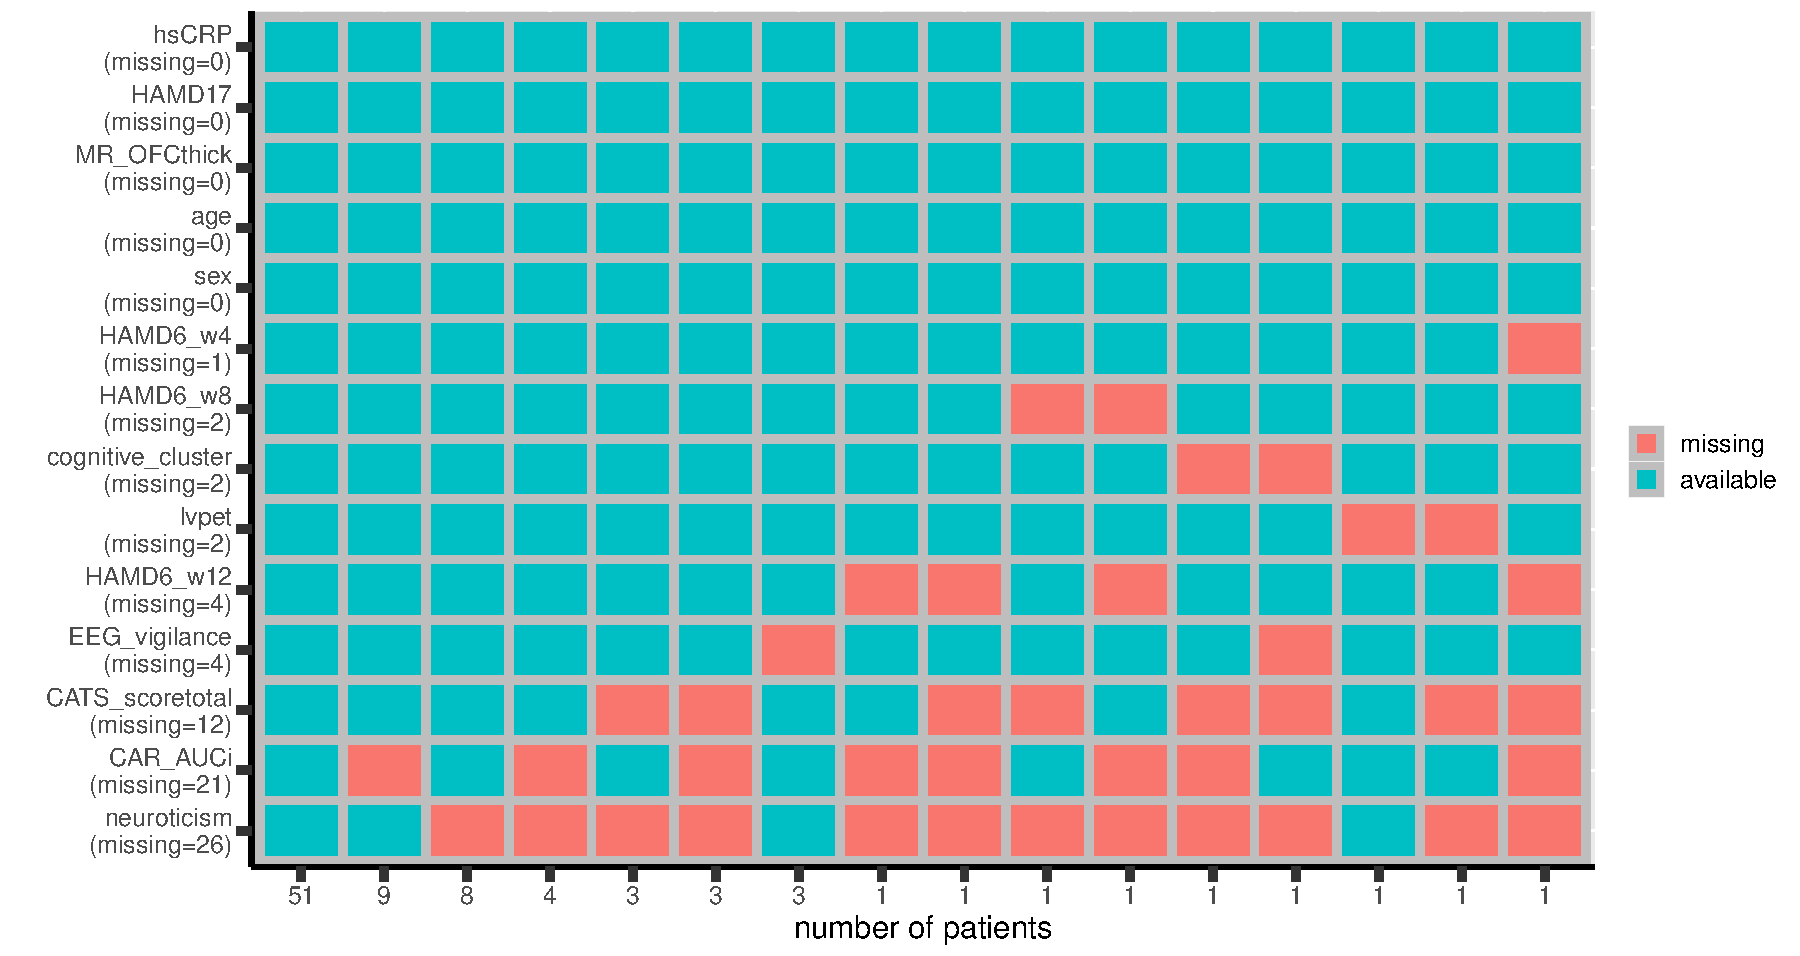
\includegraphics[trim={0 0 0 0},width=0.9\textwidth]{./figures/gg-missingPattern.pdf}
\caption{\label{fig:missingPattern}Missing data patterns}
\end{figure}

\bigskip

\subsection{Outcome trajectories}
\label{sec:org8bfd5b4}

The following table describes:
\begin{itemize}
\item at week 4: the number of patients that recovered (\texttt{nr2r}) or who did
not recovered (\texttt{nr2nr}).
\item at week 8 and 12: the number of patients who did not recover before
or at the current time (\texttt{nr2nr}), the number of patients who just
recovered (\texttt{nr2r}), the number of patients who recovered previously
but go worse (\texttt{r2nr}), and the number of patients recovered
previously and stay recovered (\texttt{r2r}). \texttt{nr2r+r2r} is then number of
patients currently classified as recovered and \texttt{nr2nr+r2nr} as not
recovered.
\end{itemize}
\begin{verbatim}
            week4       week8      week12
nr2nr 52 (58.43%) 30 (34.48%) 20 (23.53%)
r2nr       0 (0%)  9 (10.34%)   6 (7.06%)
nr2r  37 (41.57%) 20 (22.99%)    17 (20%)
r2r        0 (0%) 28 (32.18%) 42 (49.41%)
total   89 (100%)   87 (100%)   85 (100%)
\end{verbatim}


To further describe the outcome trajectory of the patients over time,
we use a latent class linear mixed model with homogeneous residual
variance-covariance between groups to identify 3 groups of
recovery. The results are shown in figure \autoref{fig:hlme} and
ressemble those of \cite{goerigk2021distinct}.

\begin{figure}[!h]
\centering
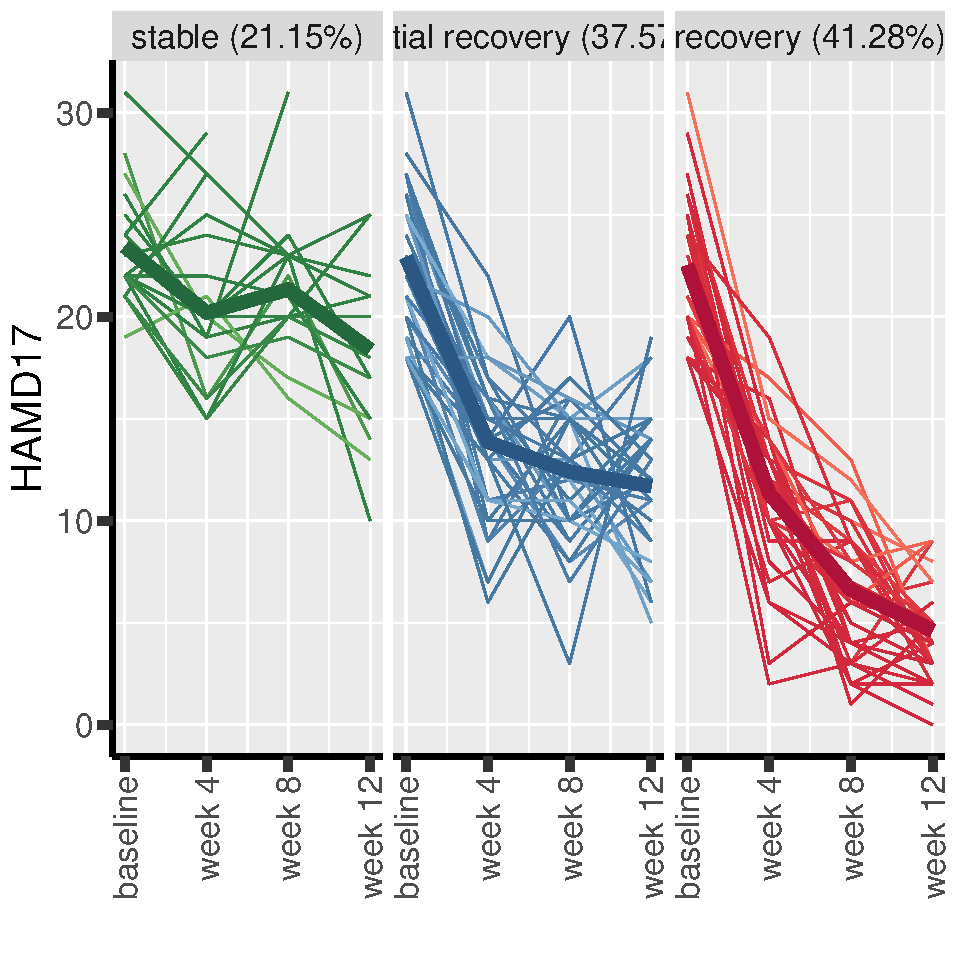
\includegraphics[trim={0 0 0 0},width=0.9\textwidth]{./figures/spaghetti-HAMD17.pdf}
\caption{\label{fig:hlme}Recovery groups found by a latent class linear mixed model (LCMM). Thin lines represent individual trajectories colored as a function of the group membership probability. Thick lines represent group trajctories estimated by the LCMM.}
\end{figure}



\subsection{Association study (linear)}
\label{sec:orga50caa6}

The following table shows the result of multiple imputation for the
logistic model with biomarkers, based on 88 patients (some with
missing biomarker values):
\begin{verbatim}
                     term    estimate    p.value adj.p.value  lower.adj upper.adj
 1:    MR (OFC thickness) -0.48611743 0.09664484  0.59435171 -1.3153682 0.3431334
 2:                HAMD17  0.32097935 0.23911230  0.91059402 -0.4554627 1.0974214
 3:                 hsCRP  0.89399954 0.17305117  0.81271604 -0.9710296 2.7590287
 4:       PET (serotonin) -0.09616763 0.71280103  0.99999133 -0.8433506 0.6510154
 5: cognition (cluster 2) -0.69912372 0.27221893  0.93996471 -2.5133247 1.1150773
 6: cognition (cluster 3) -1.87992179 0.01004351  0.09046179 -3.9211639 0.1613203
 7:       EEG (vigilance) -0.69847488 0.02015285  0.17155060 -1.5426301 0.1456804
 8:                  CATS  0.07479048 0.78655856  0.99999954 -0.7153047 0.8648857
 9:              Cortisol  0.28152530 0.34520600  0.97701174 -0.5691779 1.1322285
10:           Neuroticism  0.22612552 0.50133395  0.99819203 -0.7346358 1.1868868
11:                female -0.57753491 0.33310871          NA         NA        NA
12:                   age  0.45193136 0.16838786          NA         NA        NA
\end{verbatim}

The smallest adjusted p-value is 0.09 obtained for cognition cluster
3: being is this cluser is associated with lower remission rate
(estimate OR=0.15). The second most significant p-value is obtained for EEG.


\clearpage

\textbf{Sensitivity analysis}: we replicated this analysis at week 4:
\begin{verbatim}
                     term    estimate    p.value adj.p.value  lower.adj upper.adj
 1:    MR (OFC thickness) -0.05876414 0.81995462   0.9999999 -0.7977520 0.6802237
 2:                HAMD17  0.08812129 0.72970162   0.9999958 -0.6416895 0.8179321
 3:                 hsCRP  0.65041183 0.32292900   0.9707452 -1.2267548 2.5275784
 4:       PET (serotonin)  0.08061616 0.74715773   0.9999978 -0.6349798 0.7962121
 5: cognition (cluster 2) -0.33296344 0.58099358   0.9996948 -2.0579792 1.3920523
 6: cognition (cluster 3) -1.30528058 0.05631125   0.4105926 -3.2382481 0.6276869
 7:       EEG (vigilance) -0.10138066 0.68695947   0.9999823 -0.8211744 0.6184131
 8:                  CATS -0.28135338 0.31830848   0.9688761 -1.0857282 0.5230215
 9:              Cortisol  0.28873615 0.34775562   0.9793286 -0.5888975 1.1663698
10:           Neuroticism  0.20053395 0.52825021   0.9990415 -0.7084860 1.1095539
11:                female -1.15006496 0.04969227          NA         NA        NA
12:                   age  0.24249711 0.35893909          NA         NA        NA
\end{verbatim}

and week 12:
\begin{verbatim}
                     term    estimate    p.value adj.p.value  lower.adj  upper.adj
 1:    MR (OFC thickness) -0.87021372 0.01059592  0.09403706 -1.8211883 0.08076082
 2:                HAMD17  0.22864772 0.43895218  0.99386231 -0.6141215 1.07141690
 3:                 hsCRP  0.54170359 0.48043219  0.99698507 -1.6490589 2.73246604
 4:       PET (serotonin)  0.14969225 0.61394466  0.99981907 -0.6978764 0.99726089
 5: cognition (cluster 2) -1.23228367 0.11663155  0.65755046 -3.4576855 0.99311813
 6: cognition (cluster 3) -1.23211761 0.14918403  0.75139652 -3.6559188 1.19168357
 7:       EEG (vigilance) -0.05548535 0.85470244  0.99999999 -0.9215959 0.81062525
 8:                  CATS  0.69398065 0.04752293  0.34992677 -0.2933312 1.68129249
 9:              Cortisol  0.46282495 0.22519432  0.88903756 -0.6224248 1.54807472
10:           Neuroticism -0.02338173 0.95340882  1.00000000 -1.1674326 1.12066918
11:                female -0.91743988 0.18900657          NA         NA         NA
12:                   age  0.73697667 0.13715573          NA         NA         NA
\end{verbatim}

At week 4 we see again some evidence for cluster 3 (without adjustment
for multiple comparisons). At week 12, the most promising biomarkers
would be OFC thickness and CATS. We also replicated the analysis when
removing CATS, Cortisol, Neuroticm and using a complete case
approach. The results are summarized on the following forest plot
(\autoref{fig:forestPlot}). We note that for some variables (age,
cognition cluster 2, OFC thickness) the association seemed more and
more pronounced over the weeks.

\clearpage
\begin{figure}[!h]
\centering
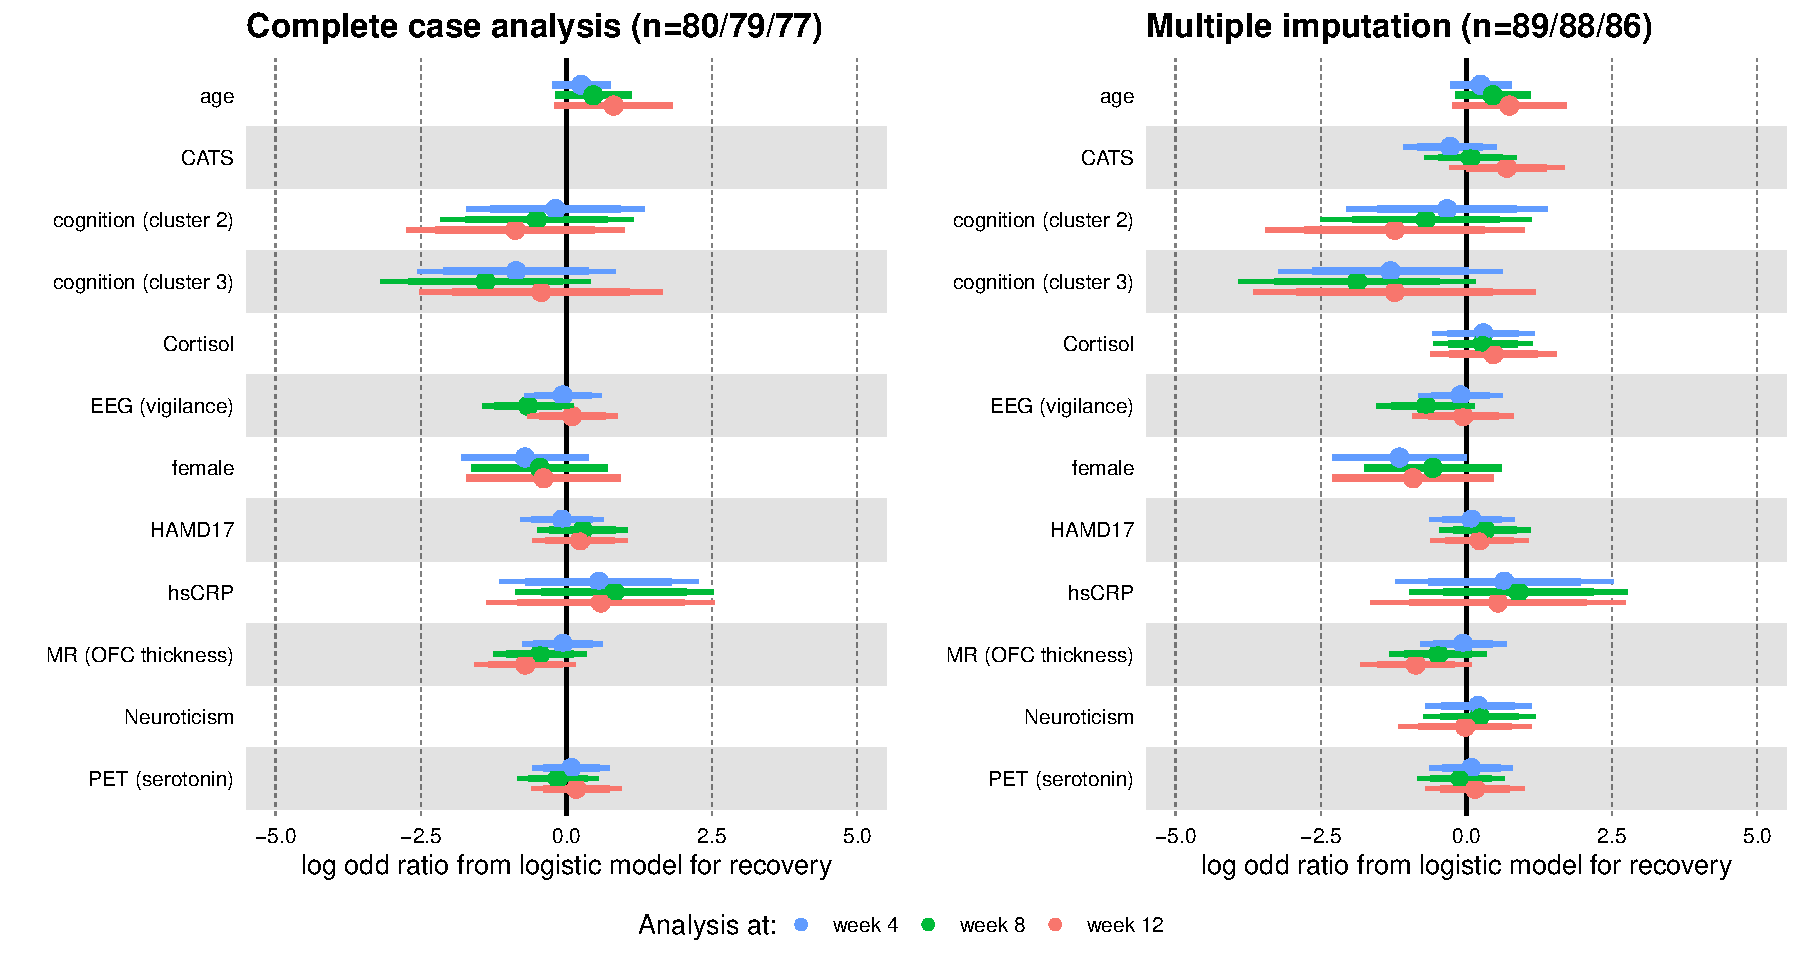
\includegraphics[trim={0 0 0 0},width=\textwidth]{./figures/gg-forestplot-OR.pdf}
\caption{\label{fig:forestPlot}Log-odd ratio estimates (full circles), confidence intervals (thick lines) and adjusted confidence intervals (thin lines) for each analysis at each timepoint. Covariates have been centered and scale to be comparable. Adjustment for multiplicity is performed over biomarkers but not over time.}
\end{figure}

\subsection{Association study (non-linear)}
\label{sec:org87f0daf}

When using random forest with the complete case approach, no biomarker
appeared relevant at week 8 (see also \autoref{fig:variableImportance}):
\begin{verbatim}
                  param              week4              week8             week12
1                female  -5e-04 (p=0.4535) -0.0047 (p=0.8501) -0.0025 (p=0.6713)
2                   age  0.0112 (p=0.1698)  0.0038 (p=0.3257)   0.004 (p=0.3407)
3    MR (OFC thickness)  0.0029 (p=0.3586)  0.0084 (p=0.2328)  0.0134 (p=0.1319)
4                HAMD17 -0.0037 (p=0.6054)  0.0025 (p=0.3646)   4e-04 (p=0.4585)
5                 hsCRP  -0.003 (p=0.7393) -0.0011 (p=0.5255) -0.0029 (p=0.7702)
6       PET (serotonin)  0.0075 (p=0.2438) -0.0073 (p=0.6933)   0.0244 (p=0.026)
7 cognition (cluster 2)  -7e-04 (p=0.4845)   5e-04 (p=0.3696)  0.0043 (p=0.1518)
8 cognition (cluster 3)  0.0093 (p=0.0629)  0.0058 (p=0.1239) -0.0026 (p=0.6643)
9       EEG (vigilance) -0.0019 (p=0.5465)  0.0034 (p=0.2527)  0.0017 (p=0.2847)
\end{verbatim}

At week 4, cognition (cluster) 3 was borderline significant. At week
12, there was some evidence for PET to be associated with the
recovery.

\begin{figure}[!h]
\centering
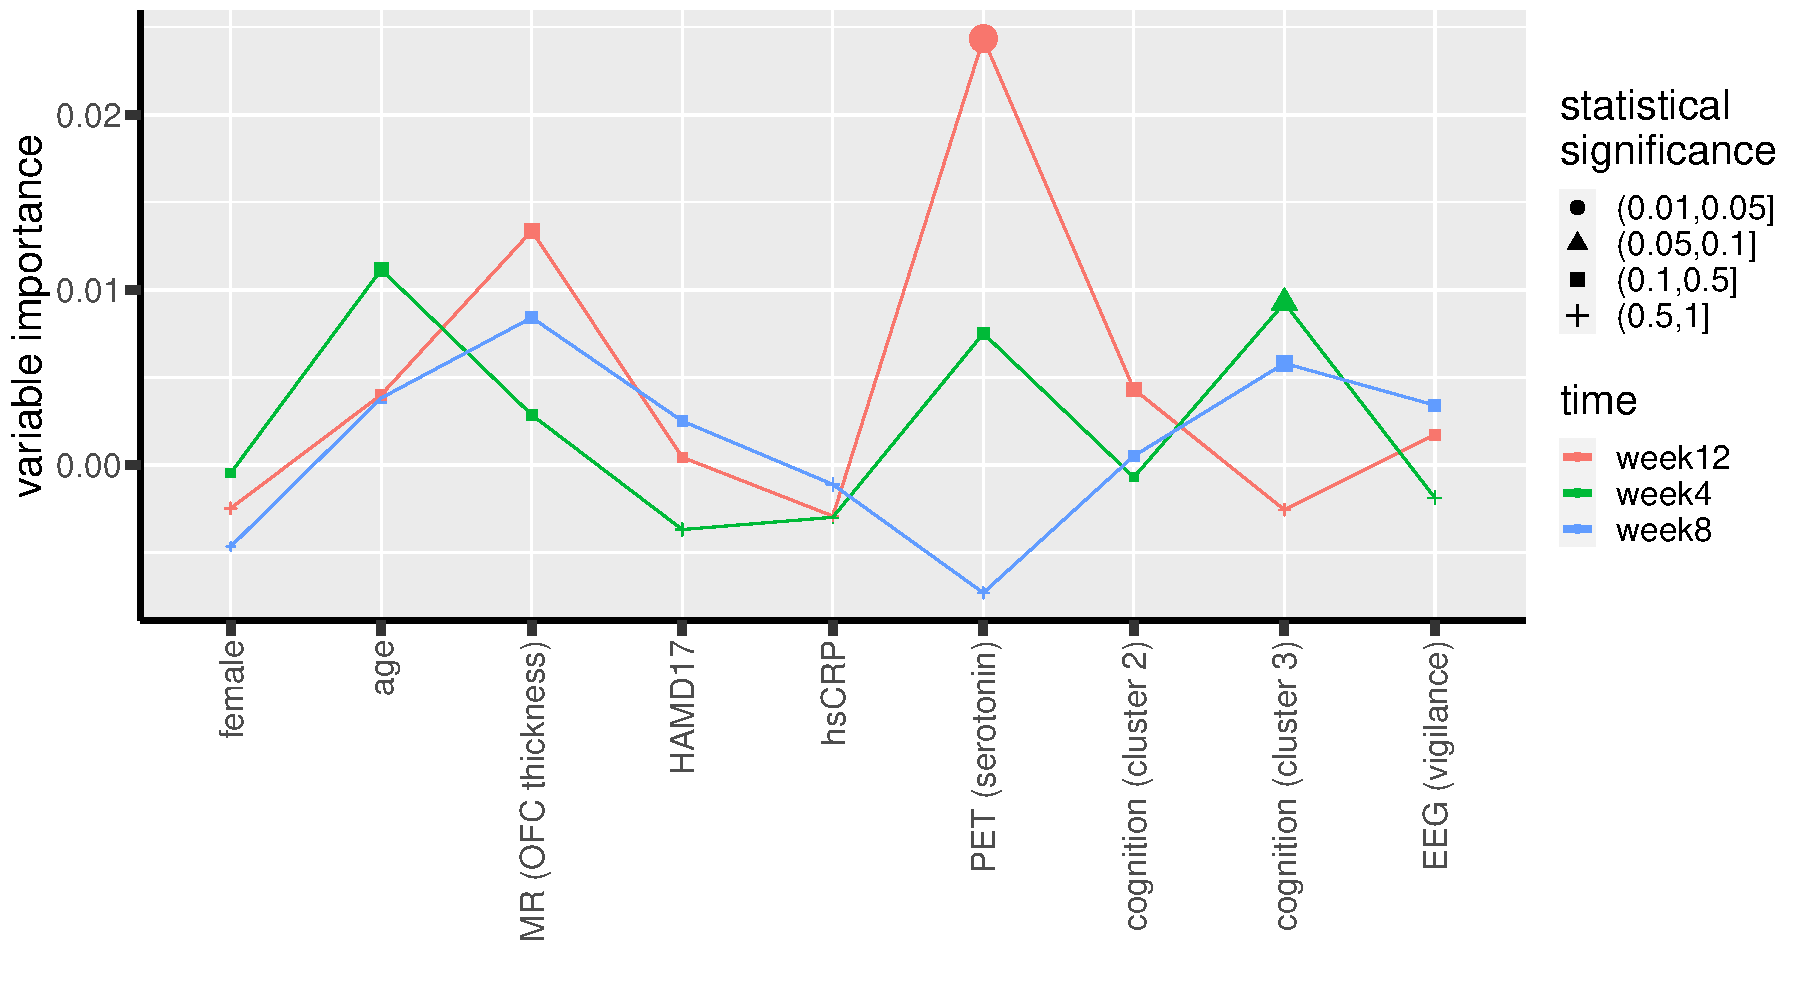
\includegraphics[trim={0 0 0 0},width=\textwidth]{./figures/variableImportance.pdf}
\caption{\label{fig:variableImportance}Log-odd ratio estimates (full circles), confidence intervals (thick lines) and adjusted confidence intervals (thin lines) for each analysis at each timepoint. Adjustment for multiplicity is performed over biomarkers but not over time.}
\end{figure}

\vfill

Further investigation using splines reveal an inverted U-shape for the
PET assocation (\autoref{fig:splineW12}, p=0.0128). A similar but non
significant association was observed for PET at week 8 (\autoref{fig:splineW8},
p=0.0904).
\vfill

\begin{figure}[!h]
\centering
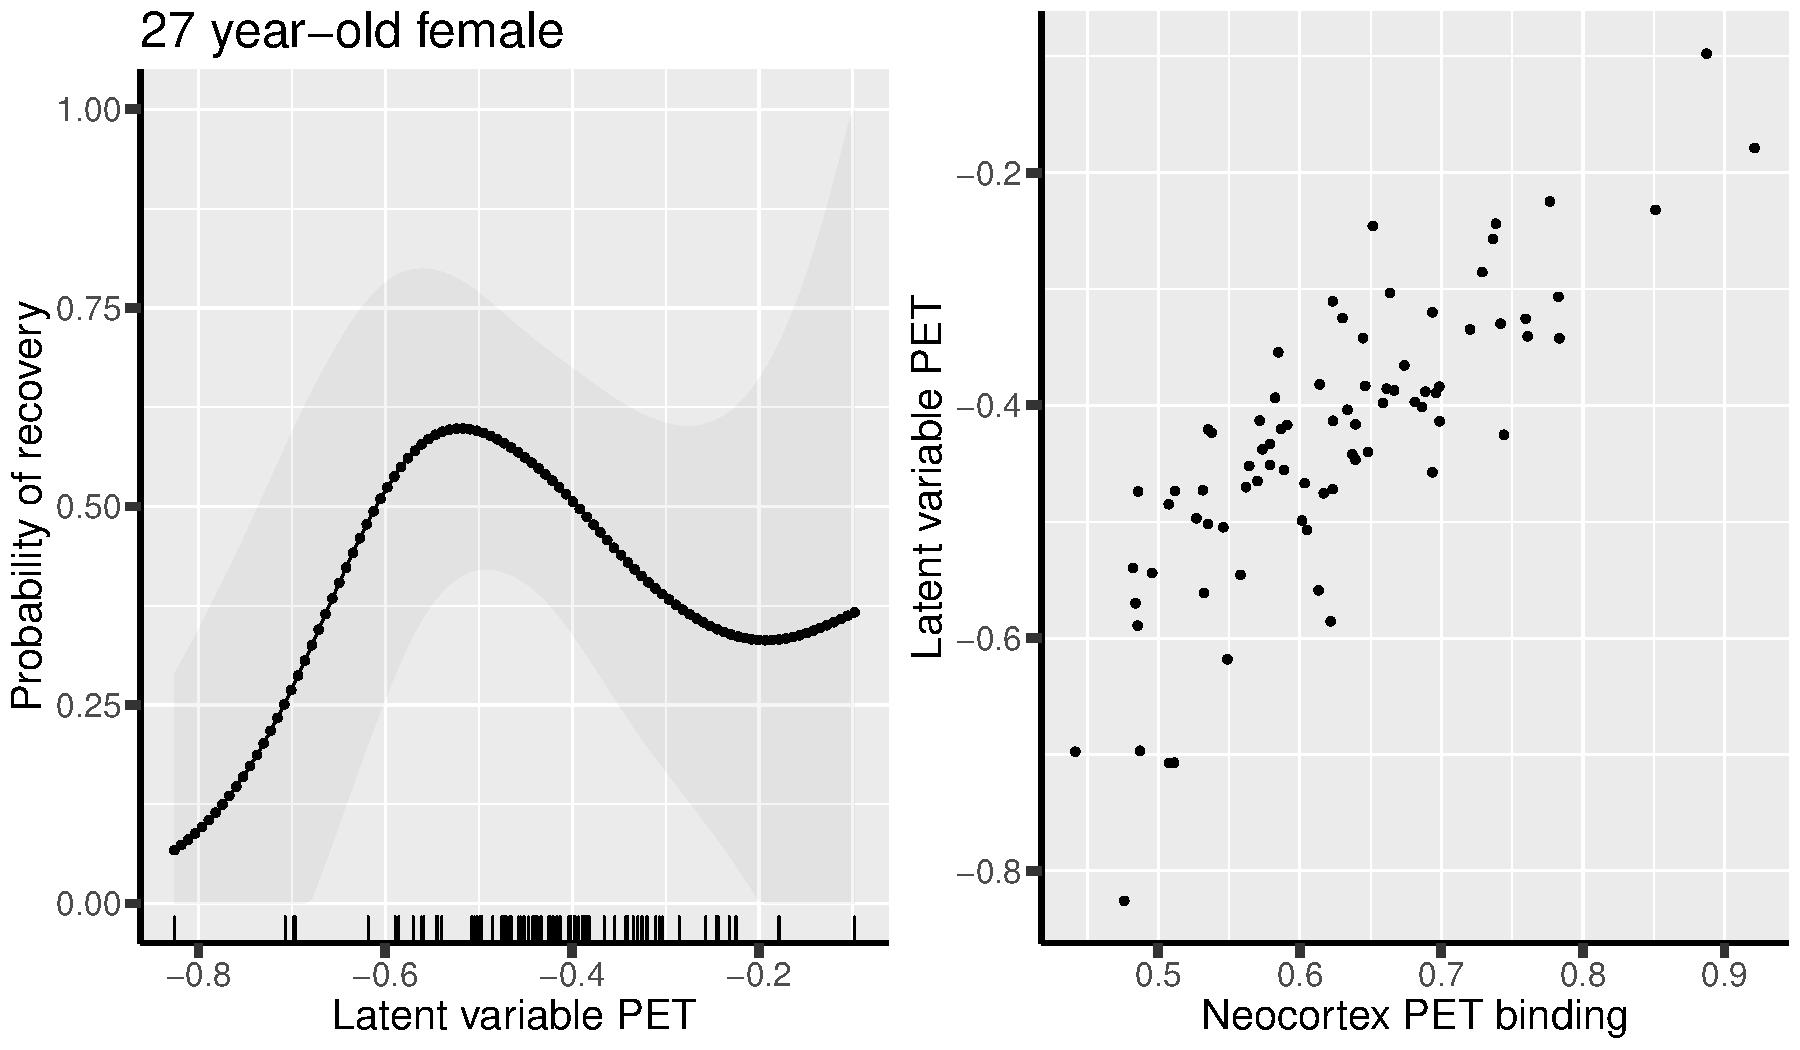
\includegraphics[trim={0 0 0 0},width=\textwidth]{./figures/gg-spline-w8.pdf}
\caption{\label{fig:splineW8}Association between recovery at week 8 and PET in a logistic model adjusted for age and sex (complete case).}
\end{figure}

\clearpage

\begin{figure}[!h]
\centering
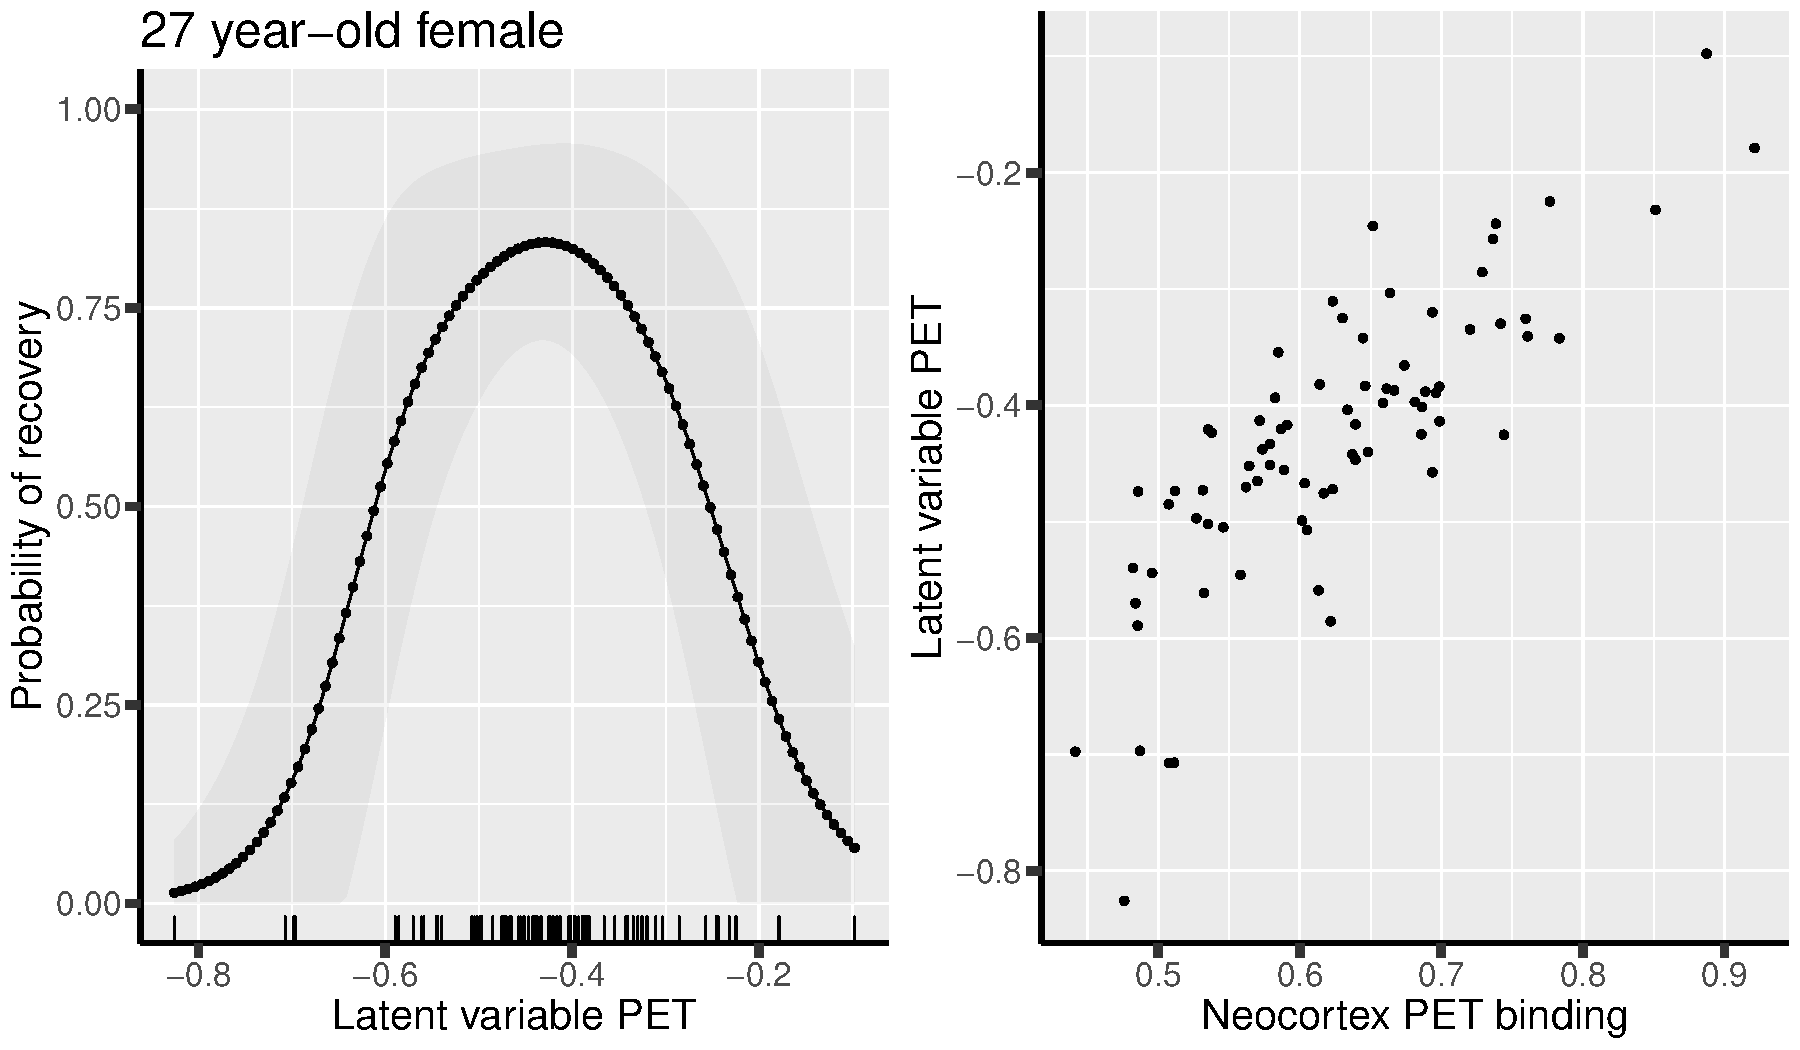
\includegraphics[trim={0 0 0 0},width=\textwidth]{./figures/gg-spline-w12.pdf}
\caption{\label{fig:splineW12}Association between recovery at week 12 and PET in a logistic model adjusted for age and sex (complete case).}
\end{figure}


\subsection{Predictive value}
\label{sec:orgb0db47d}

\autoref{fig:perfW4-dens}, \autoref{fig:perfW8-dens}, and
\autoref{fig:perfW12-dens} display the predicted probability obtain
after cross-validation colored by recovery group. Overall it looks
that the group are comparable at week 4 but there may be a difference
at week 8 and 12. The corresponding ROC curve are put in appendix
(\autoref{fig:perfW4-ROC}, \autoref{fig:perfW8-ROC},
\autoref{fig:perfW12-ROC}).

\begin{figure}[!h]
\centering
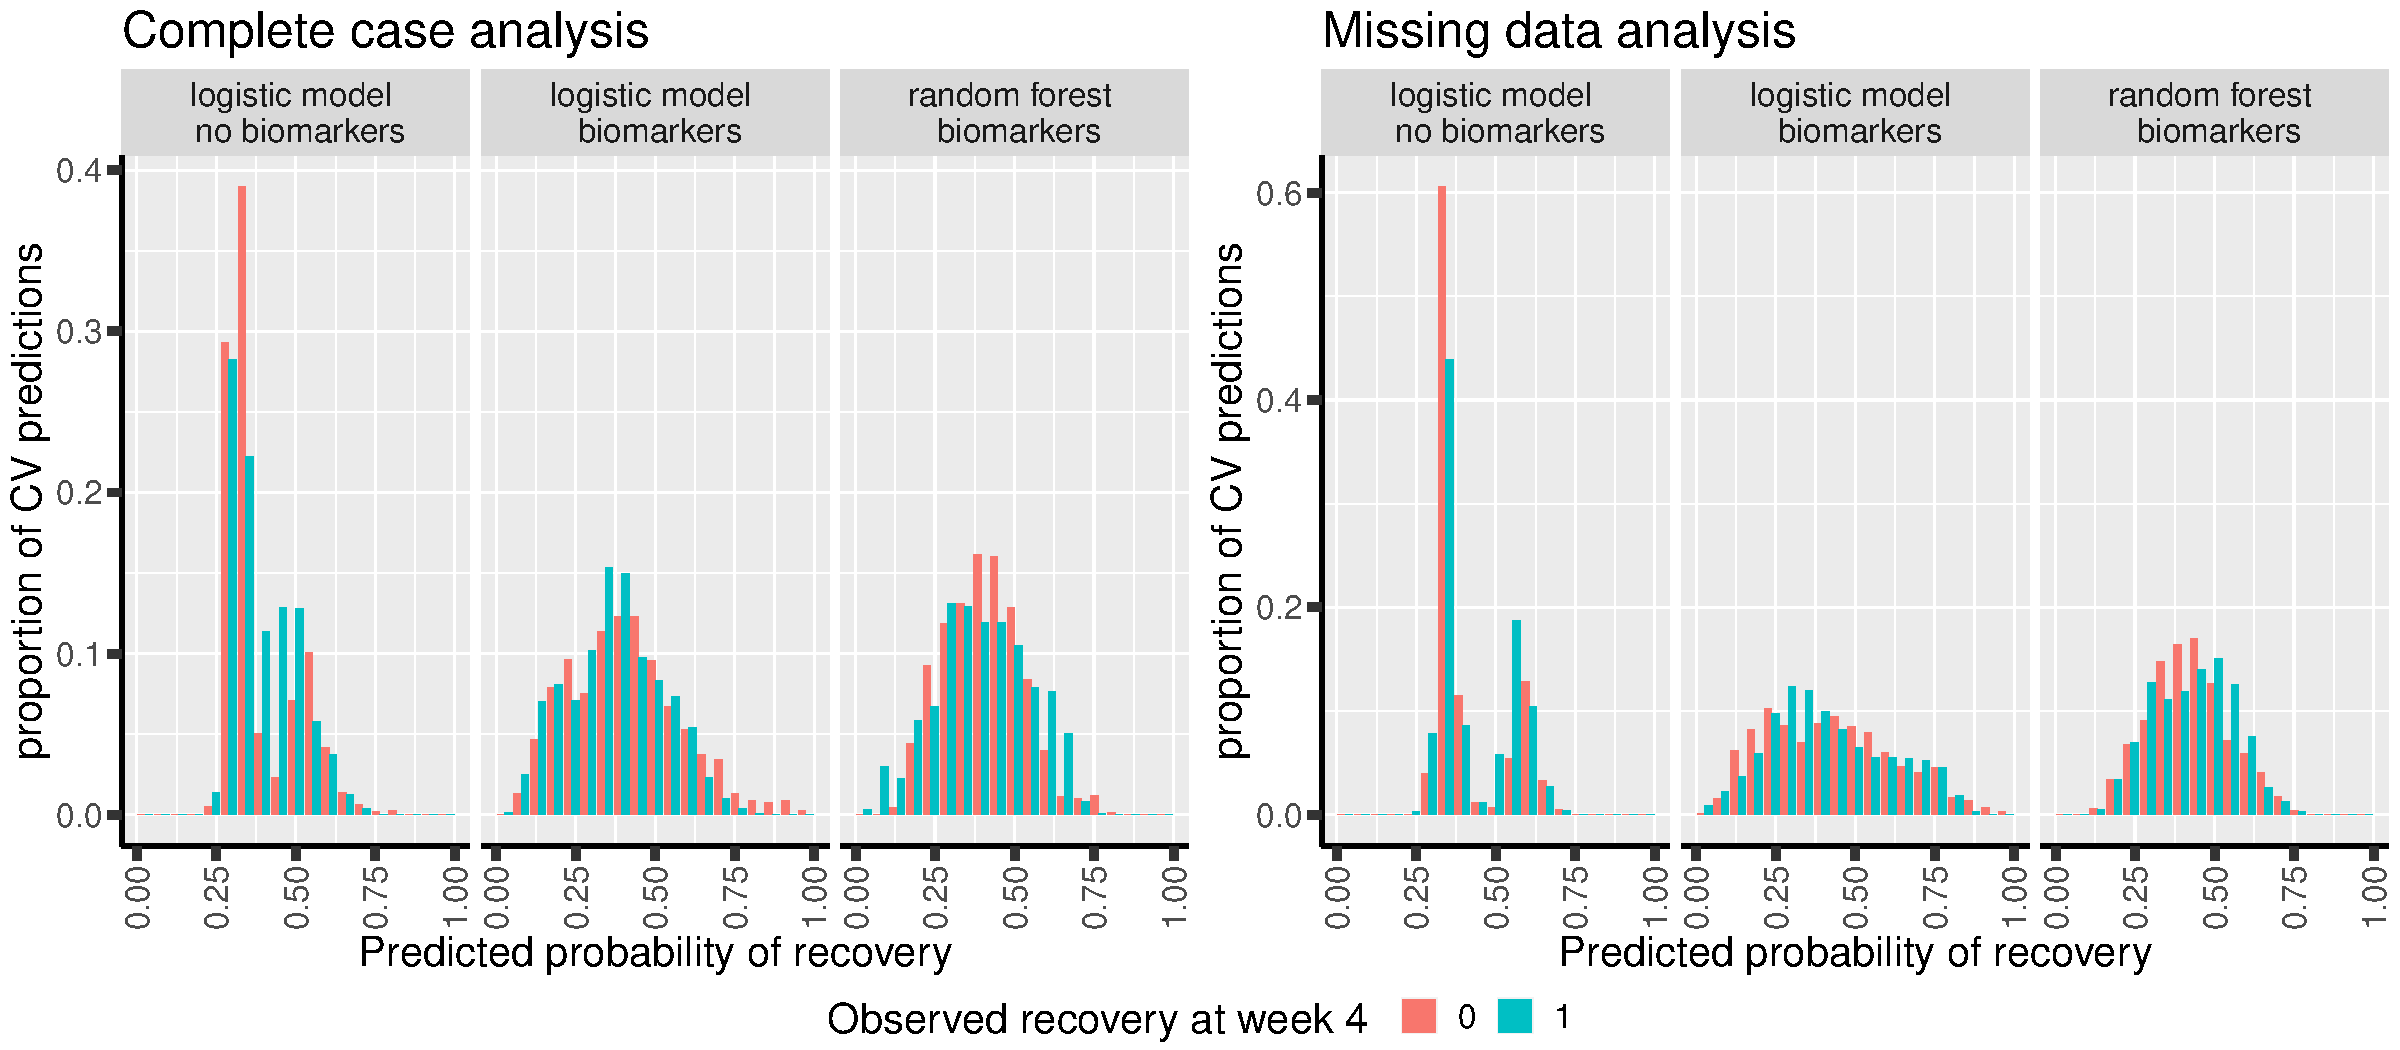
\includegraphics[trim={0 0 0 0},width=\textwidth]{./figures/hist-pred-week4.pdf}
\caption{\label{fig:perfW4-dens}Distribution of the predicted probability of recovery at week 4 per group according to each model.}
\end{figure}

\clearpage

\begin{figure}[!h]
\centering
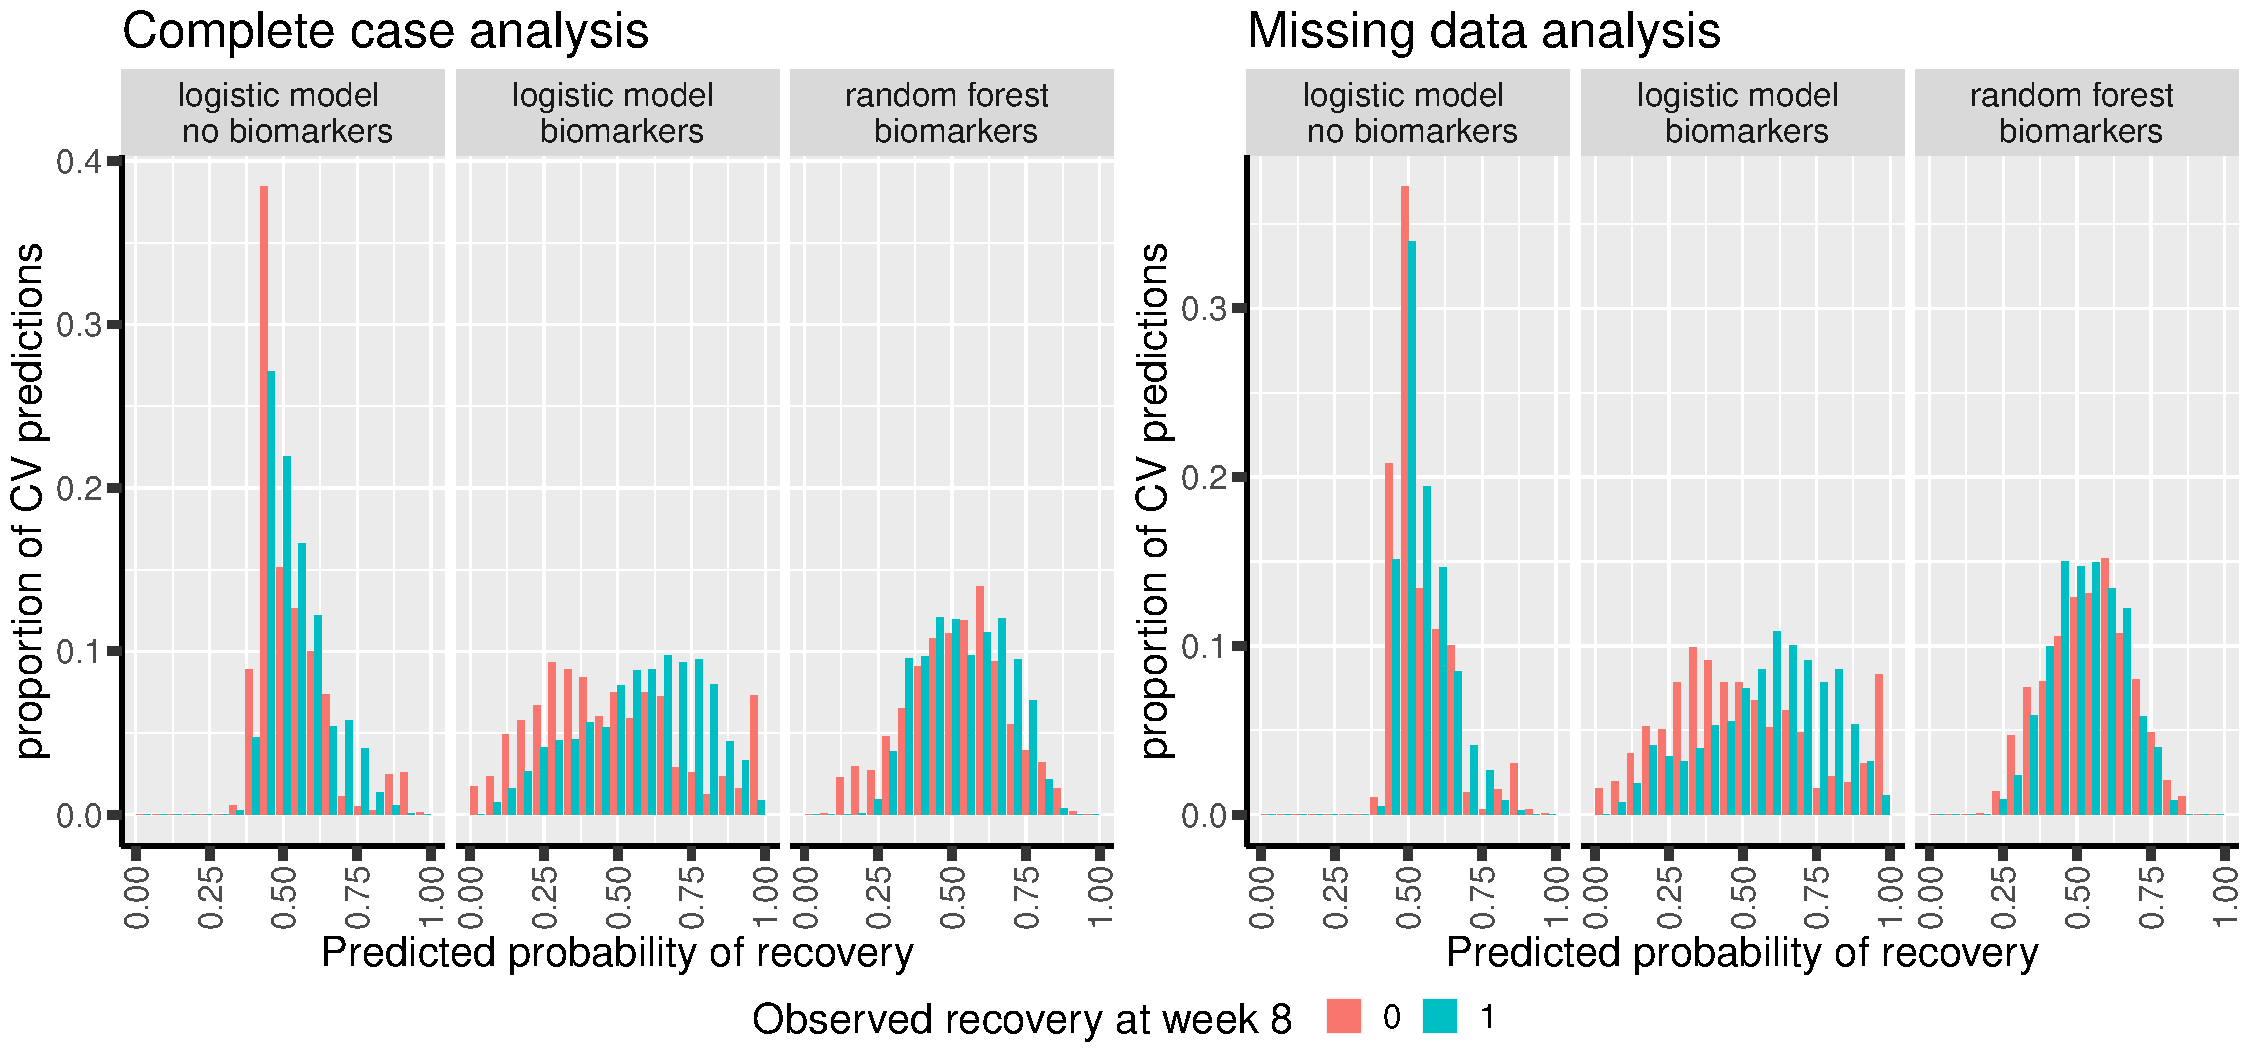
\includegraphics[trim={0 0 0 0},width=\textwidth]{./figures/hist-pred-week8.pdf}
\caption{\label{fig:perfW8-dens}Distribution of the predicted probability of recovery at week 8 per group according to each model.}
\end{figure}

\begin{figure}[!h]
\centering
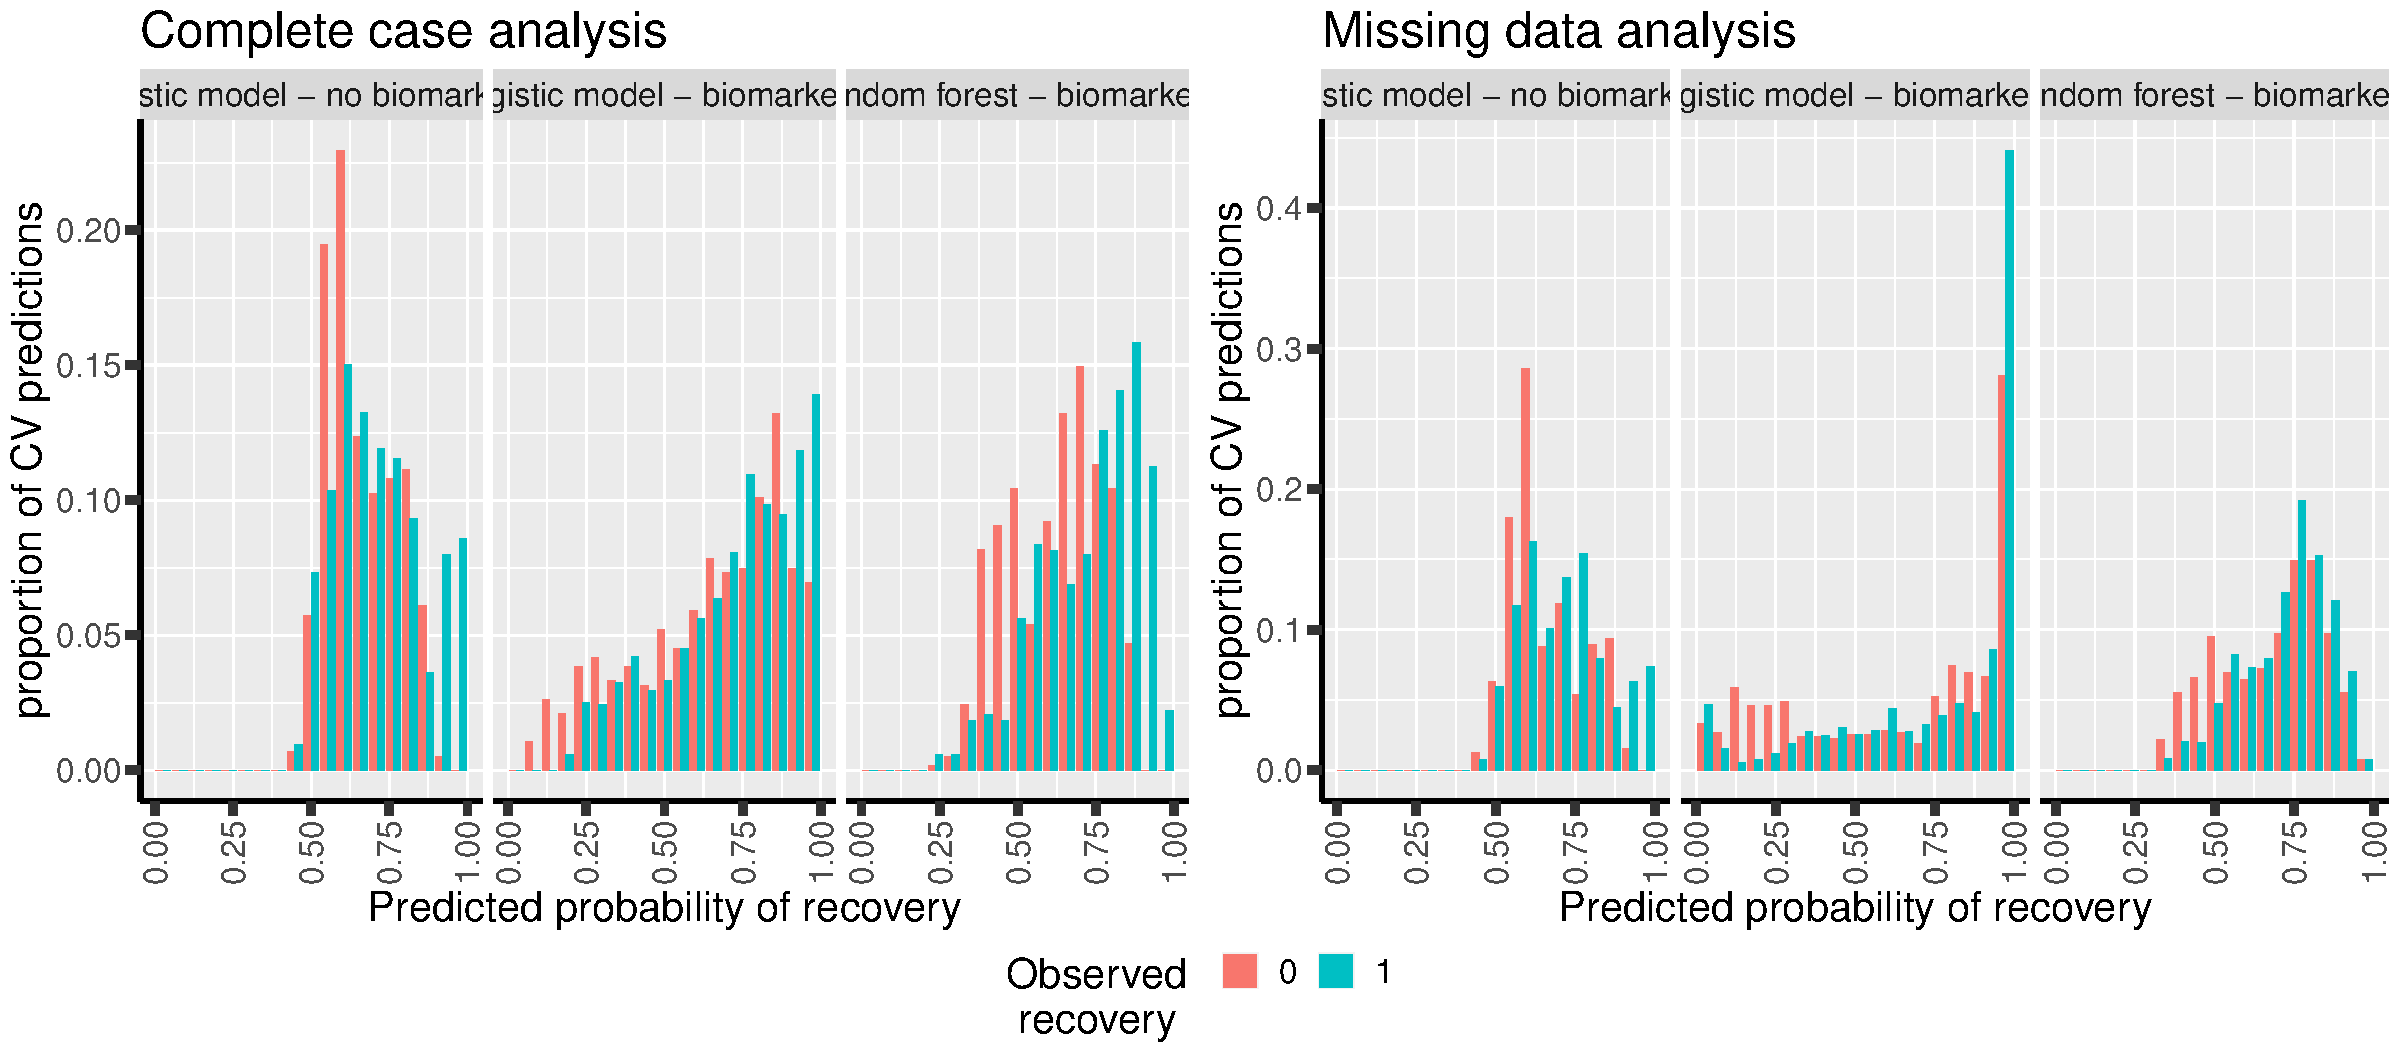
\includegraphics[trim={0 0 0 0},width=\textwidth]{./figures/hist-pred-week12.pdf}
\caption{\label{fig:perfW12-dens}Distribution of the predicted probability of recovery at week 12 per group according to each model.}
\end{figure}

The table below summarizes the predictive performance. There was some
evidence for some discriminative power of the biomarkers at week 8
(AUC=0.643, p=0.011) and 12 (AUC=0.573, p=0.119) with the logistic
regression. The calibration of these model was however not clearly
better than the null model with interept only (p=0.158 and
p=0.063).

\vfill

The point estimates of the random forest were not
superior to the logistic model (with biomarkers) in term of AUC. The
brier score was comparable to the logistic model with no biomarker.

\clearpage

\begin{verbatim}
                model week             AUC           Brier
1: GLM (no biomarker)    4 0.488 (p=0.226) 0.249 (p=0.161)
2:                       8 0.513 (p=0.162) 0.259 (p=0.352)
3:                      12 0.608 (p=0.018) 0.207 (p=0.026)
4:   GLM (biomarkers)    4 0.489 (p=0.498) 0.339 (p=0.788)
5:                       8 0.643 (p=0.011) 0.311 (p=0.158)
6:                      12 0.605 (p=0.046) 0.263 (p=0.063)
7:    RF (biomarkers)    4 0.444 (p=0.704) 0.275 (p=0.759)
8:                       8 0.462 (p=0.595) 0.274 (p=0.577)
9:                      12 0.573 (p=0.119) 0.214 (p=0.086)
\end{verbatim}

\bigskip

\textbf{Sensitivity analysis}: Similar results were obtained with the
complete case analysis (which also drop 3 biomarkers):
\begin{verbatim}
                model week             AUC           Brier
1: GLM (no biomarker)    4 0.501 (p=0.210) 0.248 (p=0.308)
2:                       8  0.56 (p=0.062) 0.255 (p=0.159)
3:                      12 0.601 (p=0.032) 0.206 (p=0.038)
4:   GLM (biomarkers)    4 0.443 (p=0.656) 0.284 (p=0.626)
5:                       8 0.637 (p=0.025) 0.253 (p=0.022)
6:                      12 0.585 (p=0.133)  0.23 (p=0.119)
7:    RF (biomarkers)    4 0.491 (p=0.444) 0.261 (p=0.466)
8:                       8 0.537 (p=0.246) 0.261 (p=0.221)
9:                      12 0.689 (p=0.011) 0.194 (p=0.016)
\end{verbatim}

The main difference being at week 12 where the RF results appeared
better (both in term of AUC and brier score) and the logistic model
worse.

\bigskip

IMPORTANT NOTE: what is missing here is a test comparing \texttt{GLM (no
biomarker)} to the other 2 models. I'm not sure yet how to do that
correctly. \newline Also some p-values are a bit weird e.g. AUC=0.501
with p=0.210. I'll double check.

\clearpage

\section{Conclusion}
\label{sec:orgee8ca91}

There is some evidence that cognition and EEG (and to a lesser extend
OFC thickness) are predictive of recovery at week 8. By some evidence,
we mean that the unadjusted p-value was significant (between 0.01 and
0.05) while the adjusted p-value was above the traditional threshold
(typically around 0.1). There was also some evidence for a predictive
value of these biomarkers: performance superior to the null predictor
and pointwise estimate of the in gain in AUC when adding the
biomarkers of about +0.13. However the Brier score was quite high and
not different from the null predictor. So while the biomarkers may
help to discriminate between patients who will recover or not, it
seems that we are not able to obtain reliable probabilities of
recovery. \newline Using a flexible model such as random forest did
not seems to help, which is to be expected with a rather limited
sample size.

\bigskip

The results were not stable over time: no biomarker appeared useful at
week 4 while at week 12 there was some evidence for OFC thickness and
a U-shape PET association with recovery. The added predictive value
was only noticeable in the complete case analysis though.

\section{References}
\label{sec:org294b126}
\begingroup
\renewcommand{\section}[2]{}
\bibliographystyle{apalike}
\bibliography{bibliography}

\endgroup

\appendix
\titleformat{\section}
{\normalfont\Large\bfseries}{Appendix~\thesection}{1em}{}

\renewcommand{\thefigure}{\Alph{figure}}
\renewcommand{\thetable}{\Alph{table}}
\renewcommand{\theequation}{\Alph{equation}}

\setcounter{figure}{0}    
\setcounter{table}{0}    
\setcounter{equation}{0}    

\setcounter{page}{1}

\clearpage

\section{ROC curves}
\label{sec:org7e7eb31}
\begin{figure}[!h]
\centering
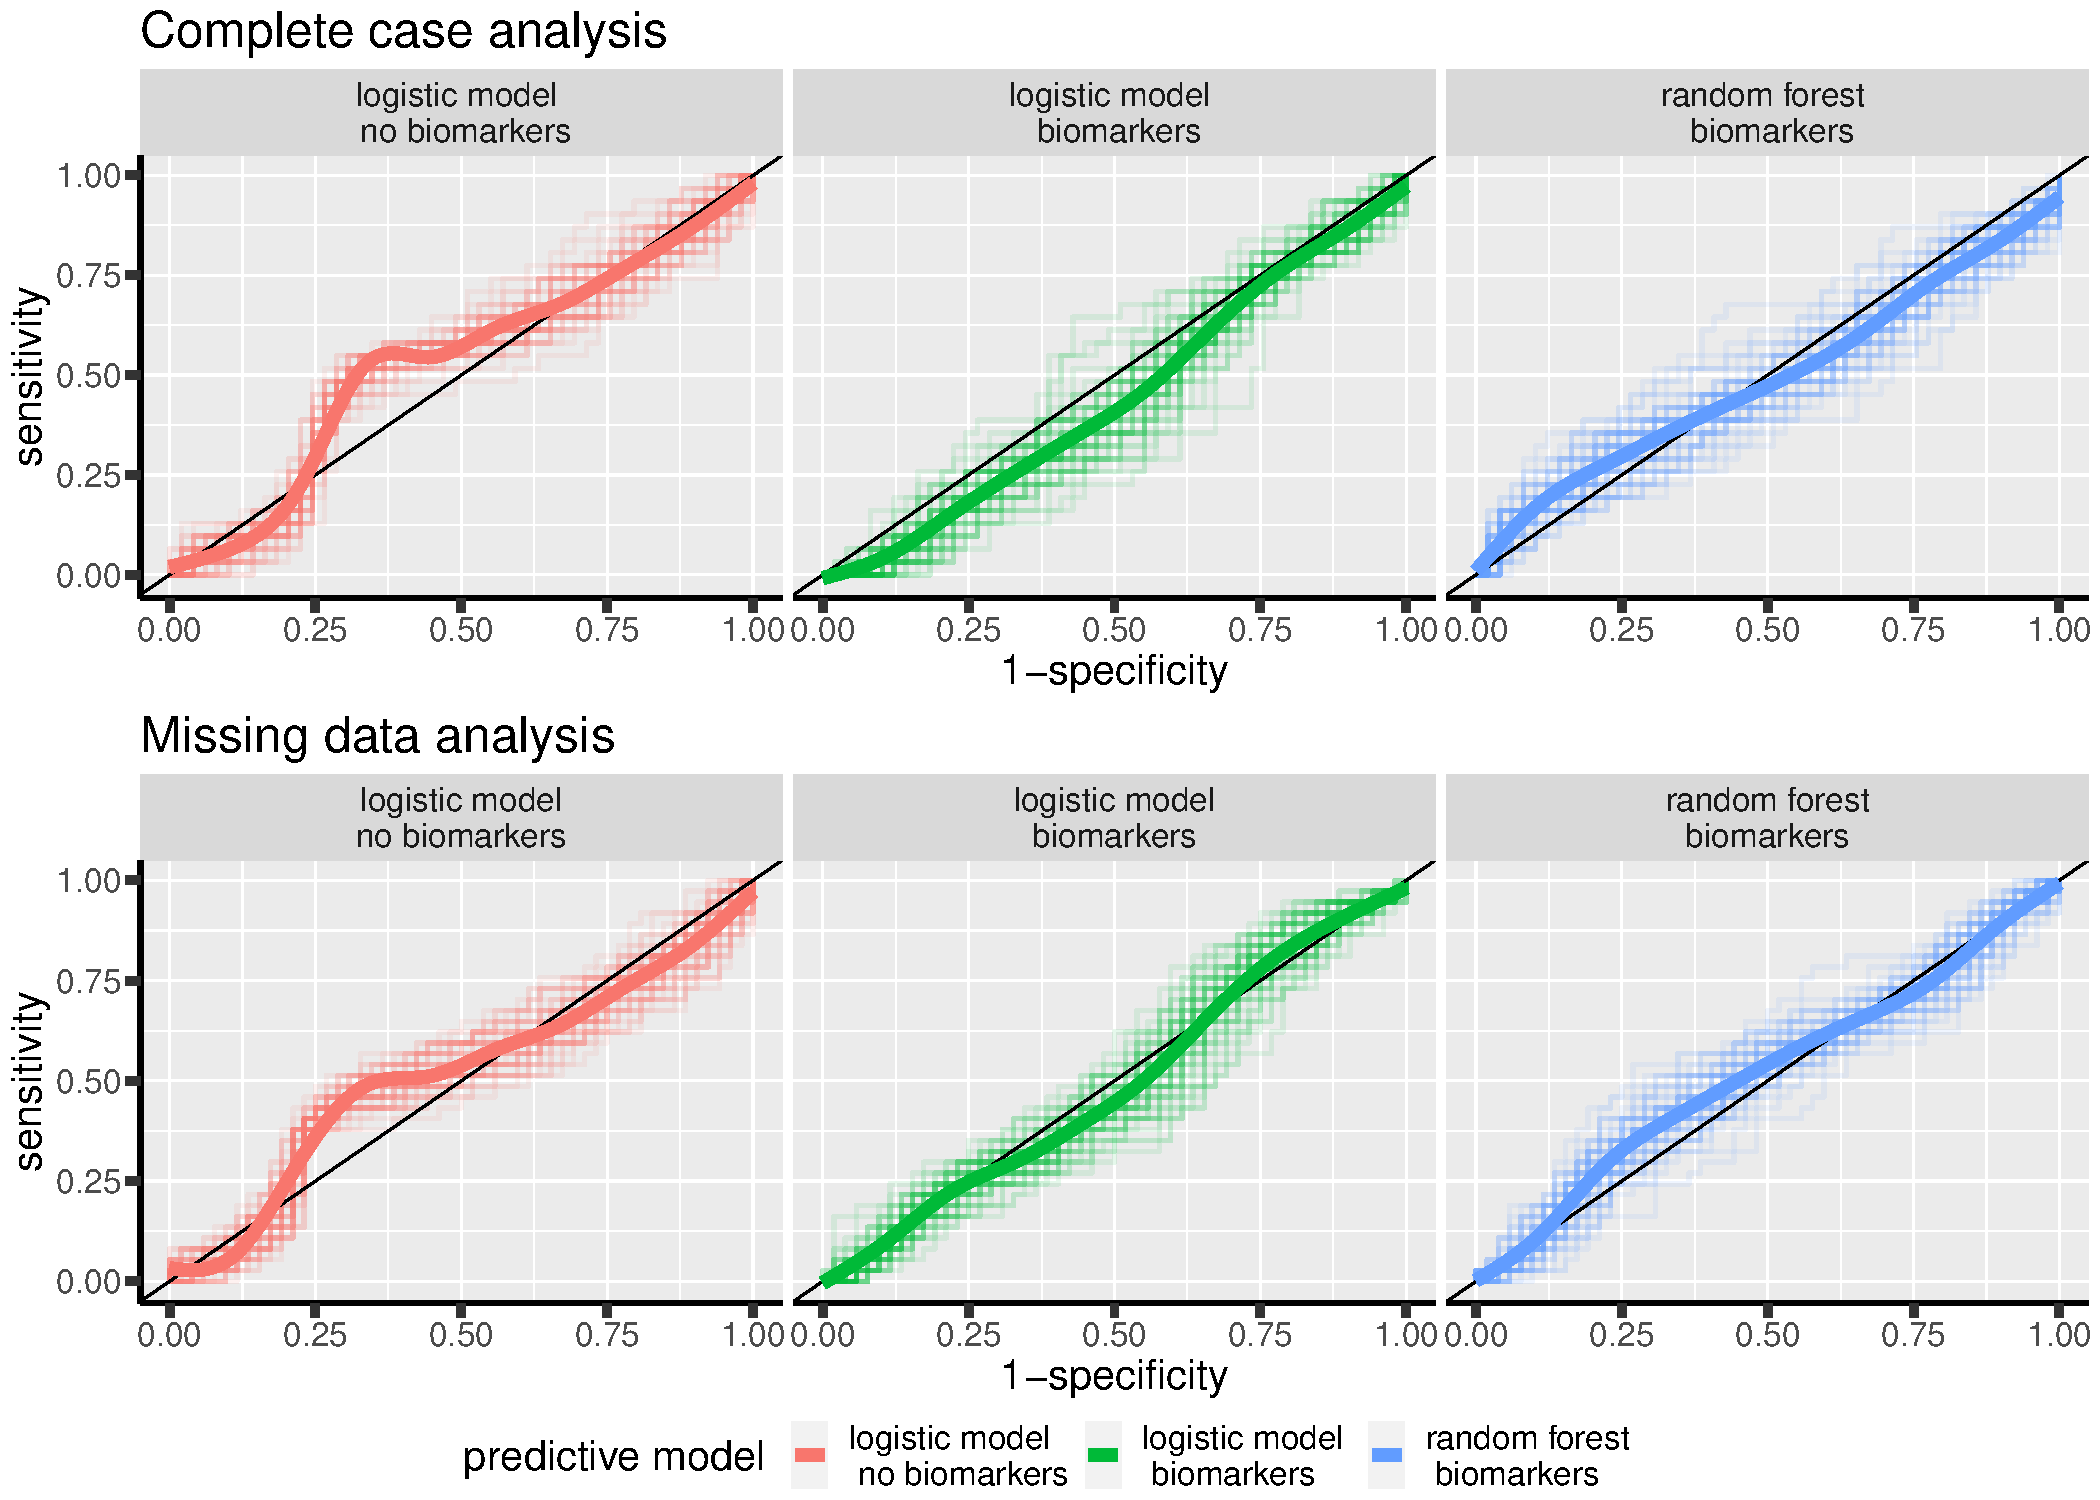
\includegraphics[trim={0 0 0 0},width=0.9\textwidth]{./figures/ROC-pred-week4.pdf}
\caption{\label{fig:perfW4-ROC}Week 4}
\end{figure}

\begin{figure}[!h]
\centering
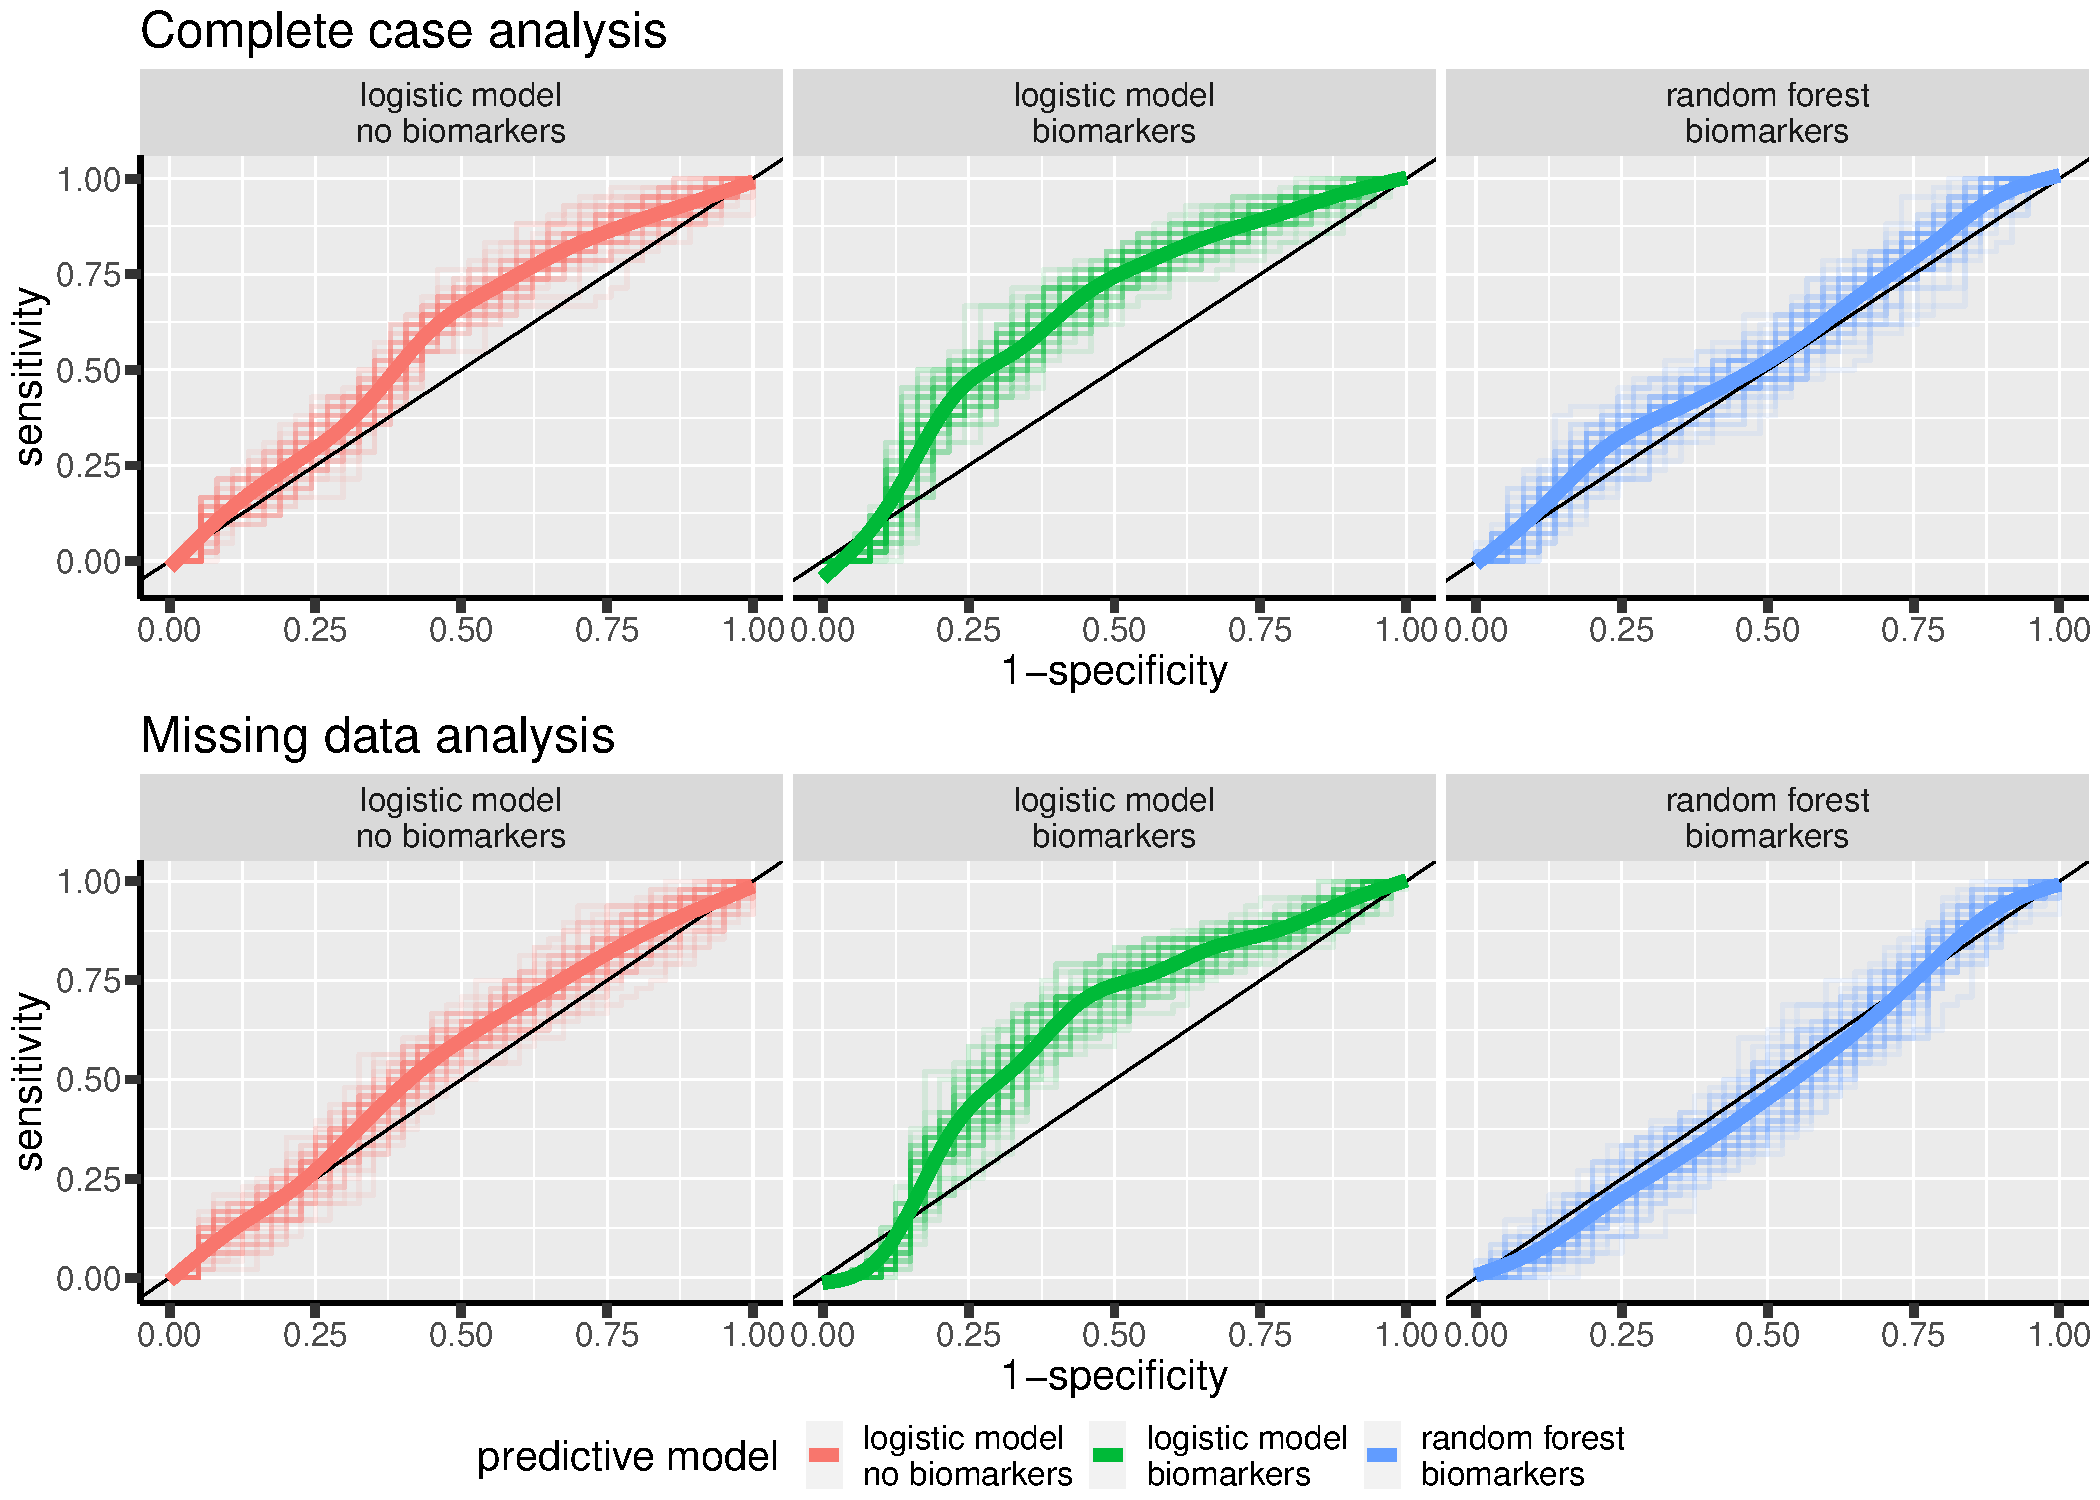
\includegraphics[trim={0 0 0 0},width=0.9\textwidth]{./figures/ROC-pred-week8.pdf}
\caption{\label{fig:perfW8-ROC}Week 8}
\end{figure}

\begin{figure}[!h]
\centering
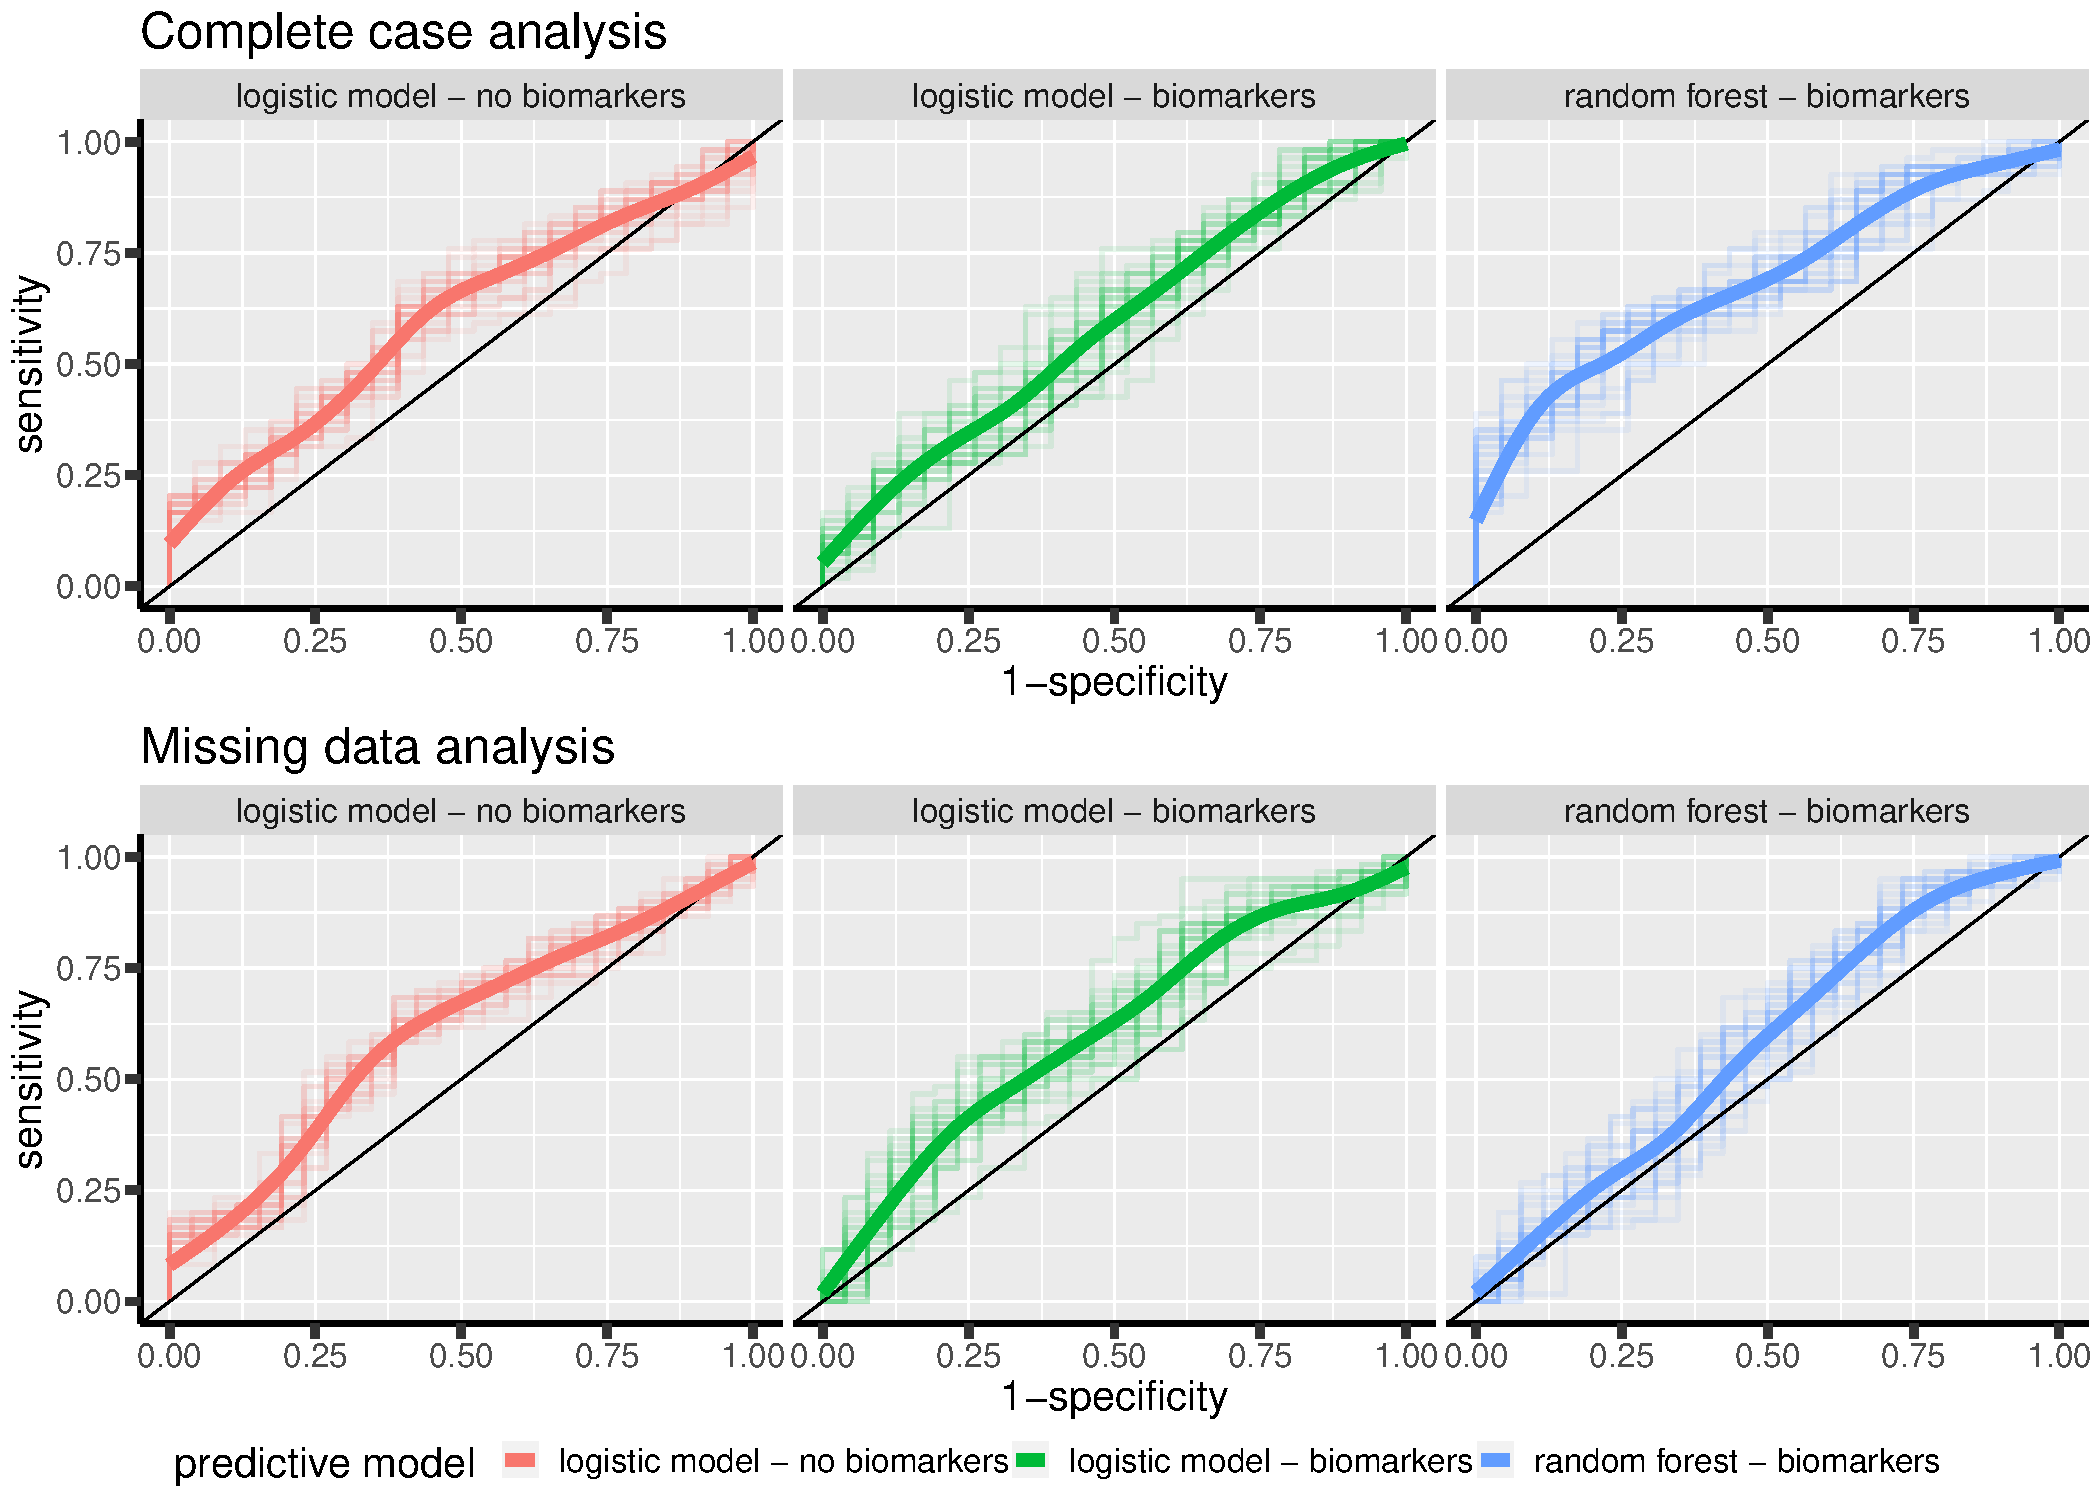
\includegraphics[trim={0 0 0 0},width=0.9\textwidth]{./figures/ROC-pred-week12.pdf}
\caption{\label{fig:perfW12-ROC}Week 12}
\end{figure}
\end{document}